\documentclass[11pt,a4paper]{article}

% ─── Packages ────────────────────────────────────────────────────
\usepackage[margin=1in]{geometry}
\usepackage{graphicx}
\usepackage{booktabs}
\usepackage{hyperref}
\usepackage{amsmath}
\usepackage{amssymb}
\usepackage{xcolor}
\usepackage{listings}
\usepackage{caption}
\usepackage{subcaption}
\usepackage{float}
\usepackage{enumitem}
\usepackage{tabularx}
\usepackage[T1]{fontenc}
\usepackage{lmodern}
\usepackage{microtype}
\usepackage{fancyhdr}
\usepackage{titlesec}
\usepackage{multirow}

% ─── Graphics path ───────────────────────────────────────────────
\graphicspath{{../plots/}}

% ─── Code listing style ─────────────────────────────────────────
\lstset{
  basicstyle=\ttfamily\small,
  breaklines=true,
  frame=single,
  backgroundcolor=\color{gray!10},
  keywordstyle=\color{blue!70!black},
  commentstyle=\color{green!50!black},
  stringstyle=\color{red!60!black},
  numbers=left,
  numberstyle=\tiny\color{gray},
  xleftmargin=2em,
}

% ─── Header/Footer ──────────────────────────────────────────────
\pagestyle{fancy}
\fancyhf{}
\fancyhead[L]{\small Profiling Kernel Scheduling Delays}
\fancyhead[R]{\small MT25037}
\fancyfoot[C]{\thepage}

% ─── Title ───────────────────────────────────────────────────────
\title{
  \textbf{Profiling Kernel Scheduling Delays Under\\Network-Intensive Workloads:}\\[0.3em]
  \Large An eBPF-Based Analysis and Mitigation Framework
}
\author{
  Rohit Kumar (MT25037)\\
  Arpit Kumar (MT25017)\\
  Abhinay Prakash (MT25010)\\
  Nindra Dhanush (MT25074)\\
  Adarsh Shukla (PhD25001)\\
  \\
  IIIT-Delhi
}
\date{March 2026}

\begin{document}

\maketitle
\thispagestyle{empty}

% ═══════════════════════════════════════════════════════════════════
% ABSTRACT
% ═══════════════════════════════════════════════════════════════════
\begin{abstract}
On commodity Linux systems under sustained network load, the kernel's softirq processing path competes directly with user-space application threads for CPU cycles, causing scheduling delays that are invisible to application-level monitoring. This project uses eBPF to instrument the Linux scheduler, softirq, and network subsystems to quantify these delays, correlate them with softirq CPU placement, and experimentally validate mitigation strategies. Through 16 controlled experiments (48 total runs) on a single-machine testbed with network namespaces and veth pairs, we vary CPU contention (via \texttt{stress-ng}), network load (via \texttt{iperf3}), softirq CPU placement (via RPS), application CPU pinning, CFS scheduler tuning, and NAPI budget parameters. Key findings: (1)~CPU contention under heavy network load causes a $27\times$ increase in p99 scheduling delay (from 149\,$\mu$s to 4,096\,$\mu$s), (2)~softirq follows socket affinity on veth rather than RPS steering (Gini coefficient 0.66--0.78), (3)~UDP and TCP produce equivalent p99 under stress (both 4,096\,$\mu$s), confirming CPU contention as the dominant factor, (4)~\texttt{SO\_BUSY\_POLL} reduces voluntary context switches by 25\% but cannot compensate for CPU starvation from \texttt{stress-ng}, and (5)~no mitigation achieved $\geq$20\% p99 improvement due to the dominant stress-ng CPU contention bottleneck. The complete instrumentation toolkit, experiment automation, raw data, and analysis scripts are provided as a reproducible package.
\end{abstract}

\tableofcontents
\newpage

% ═══════════════════════════════════════════════════════════════════
\section{Introduction}
\label{sec:intro}
% ═══════════════════════════════════════════════════════════════════

Modern Linux systems handling sustained network traffic face a fundamental contention problem: the kernel's softirq processing path---responsible for packet reception via \texttt{NET\_RX\_SOFTIRQ}, TCP/IP stack processing, and NAPI polling---competes directly with user-space application threads for CPU cycles. When softirq execution is colocated with latency-sensitive application threads, and especially when compounded by CPU contention from unrelated processes, scheduling delays escalate non-linearly. Runqueue depths grow, CFS \texttt{vruntime} accounting skews against newly-woken threads, and wakeup-to-actual-execution latency inflates from microseconds to milliseconds~\cite{dean2013tail}.

These tail-latency spikes are \emph{invisible} to application-level monitoring and can only be diagnosed through kernel-level tracing. eBPF~\cite{starovoitov2014ebpf} provides a safe, efficient mechanism to instrument the scheduler and network subsystems at tracepoint granularity without modifying kernel source code or introducing significant overhead.

This project makes the following contributions:

\begin{enumerate}[leftmargin=*]
  \item \textbf{eBPF Instrumentation Toolkit}: Five bpftrace/BCC scripts covering scheduler tracing (\texttt{sched\_wakeup}/\texttt{sched\_switch}), softirq profiling (\texttt{softirq\_entry}/\texttt{softirq\_exit}), packet drop detection, CPU migration tracking, and \texttt{/proc} metrics collection---all using in-kernel histogram aggregation for low overhead ($<$5\%).

  \item \textbf{16-Experiment Controlled Matrix}: Systematic variation of CPU contention, network load, softirq CPU placement (via RPS), application CPU pinning, CFS scheduler parameters, NAPI budget tuning, and protocol (TCP/UDP), with 3 runs per experiment (48 total).

  \item \textbf{Hypothesis-Driven Analysis}: Validation of four hypotheses about softirq colocation, CPU contention interaction effects, CFS tuning impact, and RPS effectiveness---with honest reporting of negative results and failed mitigations.

  \item \textbf{Reproducible Package}: Automated experiment runner, raw data ($\sim$960 files), 34 publication-quality plots, and analysis scripts, reproducible on any Linux 5.15+ system with $\geq$4 cores.
\end{enumerate}


% ═══════════════════════════════════════════════════════════════════
\section{Problem Statement}
\label{sec:problem}
% ═══════════════════════════════════════════════════════════════════

On commodity Linux systems under sustained network load, the kernel's softirq processing path (\texttt{NET\_RX\_SOFTIRQ}, NAPI poll, TCP/IP stack work) competes directly with user-space threads for CPU time. When softirq execution is colocated with latency-sensitive application threads---especially under CPU contention from unrelated processes---scheduling delays escalate non-linearly: runqueue depths grow, CFS \texttt{vruntime} accounting skews, and wakeup-to-execution latency inflates from microseconds to milliseconds.

These tail-latency spikes directly degrade systems such as low-latency trading pipelines and high-throughput web servers. More broadly, they produce p99 and p99.9 latency spikes that are invisible to application-level monitoring and can only be diagnosed through kernel-level tracing.

\textbf{Research Questions:}
\begin{enumerate}[leftmargin=*]
  \item At what level of network load does scheduling delay exceed 1\,ms p99 for a colocated application under default kernel configuration?
  \item Does softirq CPU placement (via RPS) meaningfully reduce scheduling delay for veth-based workloads?
  \item Which mitigation strategy (RPS, CPU pinning, CFS tuning, NAPI budget, \texttt{SO\_BUSY\_POLL}) most effectively reduces tail scheduling delay?
  \item How does the interaction between CPU contention and network load affect scheduling delay---additively or super-linearly?
\end{enumerate}


% ═══════════════════════════════════════════════════════════════════
\section{Motivation}
\label{sec:motivation}
% ═══════════════════════════════════════════════════════════════════

The gap between median and tail latency in networked services is a well-documented problem~\cite{dean2013tail, li2014tales}. While application-level profiling reveals slow requests, it cannot attribute the delay to its kernel-level root cause. A request that takes 1\,ms at the application level may have spent 900\,$\mu$s waiting in the kernel's runqueue because a softirq handler pre-empted the application's CPU.

eBPF-based instrumentation provides the missing visibility. By attaching to \texttt{sched\_wakeup} and \texttt{sched\_switch} tracepoints, we can measure the exact time a thread spends waiting in the runqueue---the ``invisible'' scheduling delay. By simultaneously tracking softirq durations and per-CPU utilization, we can attribute this delay to specific kernel subsystems.

This work is motivated by the practical need to:
\begin{itemize}[leftmargin=*]
  \item \textbf{Quantify} the scheduling cost of network processing under controlled conditions
  \item \textbf{Attribute} tail latency to specific kernel mechanisms (softirq, CFS, runqueue depth)
  \item \textbf{Evaluate} concrete mitigations available to system administrators without kernel modifications
  \item \textbf{Provide} a reproducible toolkit for diagnosing scheduling delays on any Linux system
\end{itemize}


% ═══════════════════════════════════════════════════════════════════
\section{Objectives}
\label{sec:objectives}
% ═══════════════════════════════════════════════════════════════════

\begin{enumerate}[leftmargin=*]
  \item \textbf{Quantify per-thread scheduling latency distributions} (runqueue delay from \texttt{sched\_wakeup} $\to$ \texttt{sched\_switch}) under six distinct load profiles.
  \item \textbf{Measure the causal relationship} between softirq CPU time and application scheduling delay by varying softirq CPU placement across 3 topologies (default, RPS-pinned, RPS-spread).
  \item \textbf{Build a reproducible eBPF instrumentation toolkit} ($\geq$5 scripts) with low overhead ($<$5\%) using in-kernel histogram aggregation.
  \item \textbf{Construct a 16-experiment matrix} varying CPU contention, network load, softirq placement, CPU pinning, CFS tuning, and protocol.
  \item \textbf{Produce per-experiment latency histograms and CDF plots} correlating scheduling delay with system configuration.
  \item \textbf{Identify the threshold of network load} at which scheduling delay exceeds 1\,ms p99.
  \item \textbf{Validate $\geq$4 mitigation strategies}, reporting both positive and negative results honestly.
  \item \textbf{Deliver a reproducible experiment package} (scripts, configs, raw data, analysis) re-runnable on any Linux 5.15+ system.
\end{enumerate}


% ═══════════════════════════════════════════════════════════════════
\section{Background and Related Work}
\label{sec:background}
% ═══════════════════════════════════════════════════════════════════

\subsection{Linux CFS Scheduler}

The Completely Fair Scheduler (CFS) uses virtual runtime (\texttt{vruntime}) to select the next runnable task from a red-black tree~\cite{fleming2017cfs}. Each task accumulates \texttt{vruntime} proportional to its execution time weighted by its priority. When a new task is woken (via \texttt{sched\_wakeup}), it is placed on the runqueue but must wait until the currently running task's timeslice expires or a preemption condition is met. The delay between wakeup and actual execution---the \emph{runqueue delay}---is the primary metric we measure.

Key CFS parameters affecting scheduling latency include \texttt{sched\_min\_granularity\_ns} (minimum timeslice, default 3\,ms), \texttt{sched\_wakeup\_granularity\_ns} (preemption threshold, default 4\,ms), and \texttt{sched\_latency\_ns} (target latency period, default 24\,ms).

\subsection{Softirq Processing and Network Stack}

When a network packet arrives, the NIC triggers a hardware interrupt, which schedules a \texttt{NET\_RX\_SOFTIRQ} to process the packet through the TCP/IP stack~\cite{mogul1996eliminating}. Softirq handlers run in interrupt context with higher priority than user-space threads, meaning they directly delay any colocated application.

For virtual network interfaces (veth pairs), packet delivery triggers softirq via \texttt{netif\_rx()} / NAPI polling without hardware IRQs~\cite{salim2001napi}. This means classical IRQ affinity tuning (\texttt{/proc/irq/N/smp\_affinity}) does not apply; instead, Receive Packet Steering (RPS)~\cite{rps2010} controls which CPU processes incoming packets.

\subsection{eBPF for Kernel Observability}

eBPF~\cite{starovoitov2014ebpf, brendangregg2019bpf} enables safe, verified programs to attach to kernel tracepoints and kprobes. Our instrumentation attaches to \texttt{sched\_wakeup}, \texttt{sched\_switch}, \texttt{softirq\_entry}, \texttt{softirq\_exit}, \texttt{netif\_receive\_skb}, and \texttt{kfree\_skb} tracepoints. In-kernel BPF histogram aggregation avoids per-event userspace overhead.

\subsection{Related Work}

Dean and Barroso~\cite{dean2013tail} characterized the ``tail at scale'' problem. Li et al.~\cite{li2014tales} identified OS scheduling as a major contributor. Ousterhout et al.~\cite{ousterhout2019shenango} developed Shenango for latency-sensitive core allocation, and Kaffes et al.~\cite{kaffes2019shinjuku} proposed Shinjuku for $\mu$s-scale preemptive scheduling. Our work differs by focusing on \emph{diagnosis and measurement} using only upstream kernel mechanisms (eBPF, RPS, CFS tuning) rather than custom schedulers, and by providing honest assessment of mitigation limitations on veth-based testbeds.


% ═══════════════════════════════════════════════════════════════════
\section{Methodology / System Design}
\label{sec:methodology}
% ═══════════════════════════════════════════════════════════════════

\subsection{Testbed Architecture}

All experiments run on a single machine using Linux network namespaces to isolate server and client, connected via a veth pair:

\begin{itemize}[leftmargin=*]
  \item \textbf{Server namespace} (\texttt{srv}, 10.0.0.1): runs \texttt{iperf3 -s} (primary) or \texttt{memcached} (planned)
  \item \textbf{Client namespace} (\texttt{cli}, 10.0.0.2): runs \texttt{iperf3 -c} load generator
  \item \textbf{CPU stressor}: \texttt{stress-ng --cpu N} for contention generation
  \item \textbf{eBPF probes}: system-wide bpftrace scripts + \texttt{/proc} pollers
\end{itemize}

\textbf{Hardware:} 8 CPU cores, 16\,GB RAM, Ubuntu 22.04 LTS, kernel 6.17.0-14-generic with BTF support.

\textbf{Why veth + namespaces:} Eliminates NIC hardware variability, ensures reproducibility, and still exercises the full kernel network stack. The veth pair generates real softirq load via \texttt{NET\_RX\_SOFTIRQ}.

\subsection{eBPF Instrumentation Toolkit}

Five instrumentation scripts collect complementary metrics:

\begin{enumerate}[leftmargin=*]
  \item \textbf{\texttt{24\_sched\_delay.bt}}: Attaches to \texttt{sched\_wakeup} and \texttt{sched\_switch} tracepoints. Records wakeup timestamp in a BPF hash map; on switch, computes $\Delta = t_{\text{switch}} - t_{\text{wakeup}}$. Primary output: in-kernel histogram (zero userspace overhead). Secondary: 1-in-1000 sampled CSV for spot-checking.

  \item \textbf{\texttt{24\_softirq\_net.bt}}: Tracks \texttt{softirq\_entry}/\texttt{softirq\_exit} for NET\_RX (vec=3) and NET\_TX (vec=2). Computes per-CPU softirq time fraction as $\text{softirq\%} = \sum(\text{duration\_us}) / \text{wall\_clock\_us} \times 100$. Includes orphaned-event guards (overwrite on re-entry, discard $>$500\,ms durations).

  \item \textbf{\texttt{24\_net\_drops.bt}}: Monitors \texttt{kfree\_skb} for packet drops and \texttt{tcp\_retransmit\_skb} for TCP retransmissions.

  \item \textbf{\texttt{24\_cpu\_migrations.bt}}: Tracks \texttt{sched\_migrate\_task} events with per-process and per-CPU-pair counts.

  \item \textbf{\texttt{24\_proc\_pollers.sh}}: Collects \texttt{/proc/stat} (per-CPU utilization), \texttt{/proc/net/softnet\_stat} (processed, dropped, time\_squeeze), \texttt{/proc/net/snmp} (TCP retransmissions), \texttt{/proc/net/sockstat} (socket memory), and interrupt snapshots at 1-second intervals.
\end{enumerate}

\subsection{Experiment Matrix}

Table~\ref{tab:experiments} shows the 16-experiment matrix. Each experiment is executed 3 times with 60\,s measurement duration, 2\,s settle time, and 10\,s cooldown between runs.

\begin{table}[H]
\centering
\caption{Experiment matrix: 16 experiments $\times$ 3 runs = 48 total runs.}
\label{tab:experiments}
\small
\begin{tabularx}{\textwidth}{l l l l l l l X}
\toprule
\textbf{Exp} & \textbf{CPU} & \textbf{Net} & \textbf{RPS} & \textbf{Pin} & \textbf{CFS} & \textbf{Proto} & \textbf{Purpose} \\
\midrule
E1  & None   & Low  & Default & None & Default & TCP & Baseline \\
E2  & None   & High & Default & None & Default & TCP & Net load only \\
E3  & Heavy  & Low  & Default & None & Default & TCP & CPU stress only \\
E4  & Heavy  & High & Default & None & Default & TCP & Worst case \\
\midrule
E5  & Heavy  & High & CPU 0   & None & Default & TCP & RPS pinned \\
E6  & Heavy  & High & All     & None & Default & TCP & RPS spread \\
E7  & Heavy  & High & Default & 2,3  & Default & TCP & App pinned \\
E8  & Heavy  & High & CPU 0   & 2,3  & Default & TCP & RPS + pin \\
\midrule
E9  & Heavy  & High & Default & None & Lowlat  & TCP & CFS tuning \\
E10 & Heavy  & High & Default & None & Default & TCP & ksoftirqd \\
E11 & None   & High & Default & None & Default & UDP & UDP baseline \\
E12 & Heavy  & High & Default & None & Default & UDP & UDP + stress \\
\midrule
E13 & Moderate & High & Default & None & Default & TCP & Threshold \\
E14 & Heavy  & High & All     & 2,3  & Lowlat  & TCP & Combined \\
E15 & Heavy  & High & All     & None & Default & TCP & RPS+bpoll \\
E16 & Heavy  & High & Default & None & Default & TCP & bpoll only \\
\bottomrule
\end{tabularx}
\end{table}

\subsection{Mitigations Tested}

Five mitigation strategies were experimentally evaluated:

\begin{description}[leftmargin=*]
  \item[M1: RPS (Receive Packet Steering)] Controls which CPU processes \texttt{NET\_RX\_SOFTIRQ} via \texttt{rps\_cpus}. Tested as pinned-to-CPU-0 (E5) and spread-across-all (E6).
  \item[M2: Application CPU Pinning] Pins application threads to CPUs 2,3 via \texttt{taskset} to isolate from softirq (E7, E8).
  \item[M3: CFS Low-Latency Tuning] Reduces \texttt{sched\_min\_granularity\_ns} to 1\,ms and \texttt{sched\_wakeup\_granularity\_ns} to 0.5\,ms for faster preemption (E9).
  \item[M4: Forced ksoftirqd] Reduces \texttt{netdev\_budget} to 50 to force softirq deferral to schedulable \texttt{ksoftirqd} threads (E10).
  \item[M5: \texttt{SO\_BUSY\_POLL}] Application-level busy polling to bypass softirq path. Uses a custom echo server since \texttt{SO\_BUSY\_POLL} requires per-socket \texttt{setsockopt} (E15, E16).
\end{description}

\subsection{Hypotheses}

\begin{description}[leftmargin=*]
  \item[H1 (Softirq Colocation):] When \texttt{NET\_RX} softirq runs on the same CPU as application threads, runqueue delay increases by $\geq$5$\times$ vs.\ separate CPUs. \emph{E4 vs.\ E8.}
  \item[H2 (Super-Linear Interaction):] Under high network load, adding CPU contention increases scheduling delay super-linearly: $\text{delay}(E4) > \text{delay}(E2) + \text{delay}(E3)$.
  \item[H3 (CFS Tuning):] Low-latency CFS parameters reduce p99 by $\geq$30\% at the cost of $\leq$5\% throughput.
  \item[H4 (RPS Distribution):] RPS across all CPUs reduces max per-CPU softirq fraction by $\geq$50\%.
\end{description}


% ═══════════════════════════════════════════════════════════════════
\section{Implementation}
\label{sec:implementation}
% ═══════════════════════════════════════════════════════════════════

\subsection{Testbed Setup Script}

\texttt{24\_setup\_testbed.sh} creates two network namespaces (\texttt{srv}, \texttt{cli}) connected via a veth pair with IPs 10.0.0.1/24 and 10.0.0.2/24. It sets MTU to 1500, \texttt{txqueuelen} to 10000, and verifies connectivity. Throughput across the veth pair reaches 88\,Gbps.

\subsection{Experiment Orchestration}

\texttt{24\_run\_experiment.sh} accepts 10 CLI parameters and orchestrates a single experiment:
\begin{enumerate}[leftmargin=*]
  \item Saves sysctl defaults (\texttt{sched\_*}, \texttt{netdev\_budget*})
  \item Applies system configuration (RPS via \texttt{rps\_cpus}, CFS via \texttt{/proc/sys/kernel/sched\_*}, NAPI budget)
  \item Starts iperf3 server in \texttt{srv} namespace
  \item Launches all 5 eBPF/proc probes in parallel
  \item Starts CPU stressor (\texttt{stress-ng}) if applicable
  \item Waits 2\,s settle $+$ 60\,s measurement
  \item Stops all processes, saves metadata JSON, restores sysctl
\end{enumerate}

Each run produces 20 output files: sampled CSVs, raw histograms, summary files, proc poller CSVs, iperf3 JSON, metadata, and sysctl backup.

\texttt{24\_run\_all\_experiments.sh} invokes all 16 experiments with 3 runs each, with parameters matching the blueprint matrix.

\subsection{Analysis Pipeline}

\begin{itemize}[leftmargin=*]
  \item \texttt{24\_parse\_histograms.py}: Parses bpftrace histogram text output to extract percentile values and generate CDFs.
  \item \texttt{24\_generate\_plots.py}: Computes derived metrics (p50/p90/p99/p99.9, softirq CPU\%, context switches, Gini coefficient) and produces 15+ plots.
  \item \texttt{24\_validate\_h\{1,2\_h3,4\}.py}: Per-hypothesis analysis with specific comparisons and plots.
\end{itemize}


% ═══════════════════════════════════════════════════════════════════
\section{Evaluation and Observations}
\label{sec:results}
% ═══════════════════════════════════════════════════════════════════

\subsection{Baseline Results (E1--E4)}

\begin{figure}[H]
  \centering
  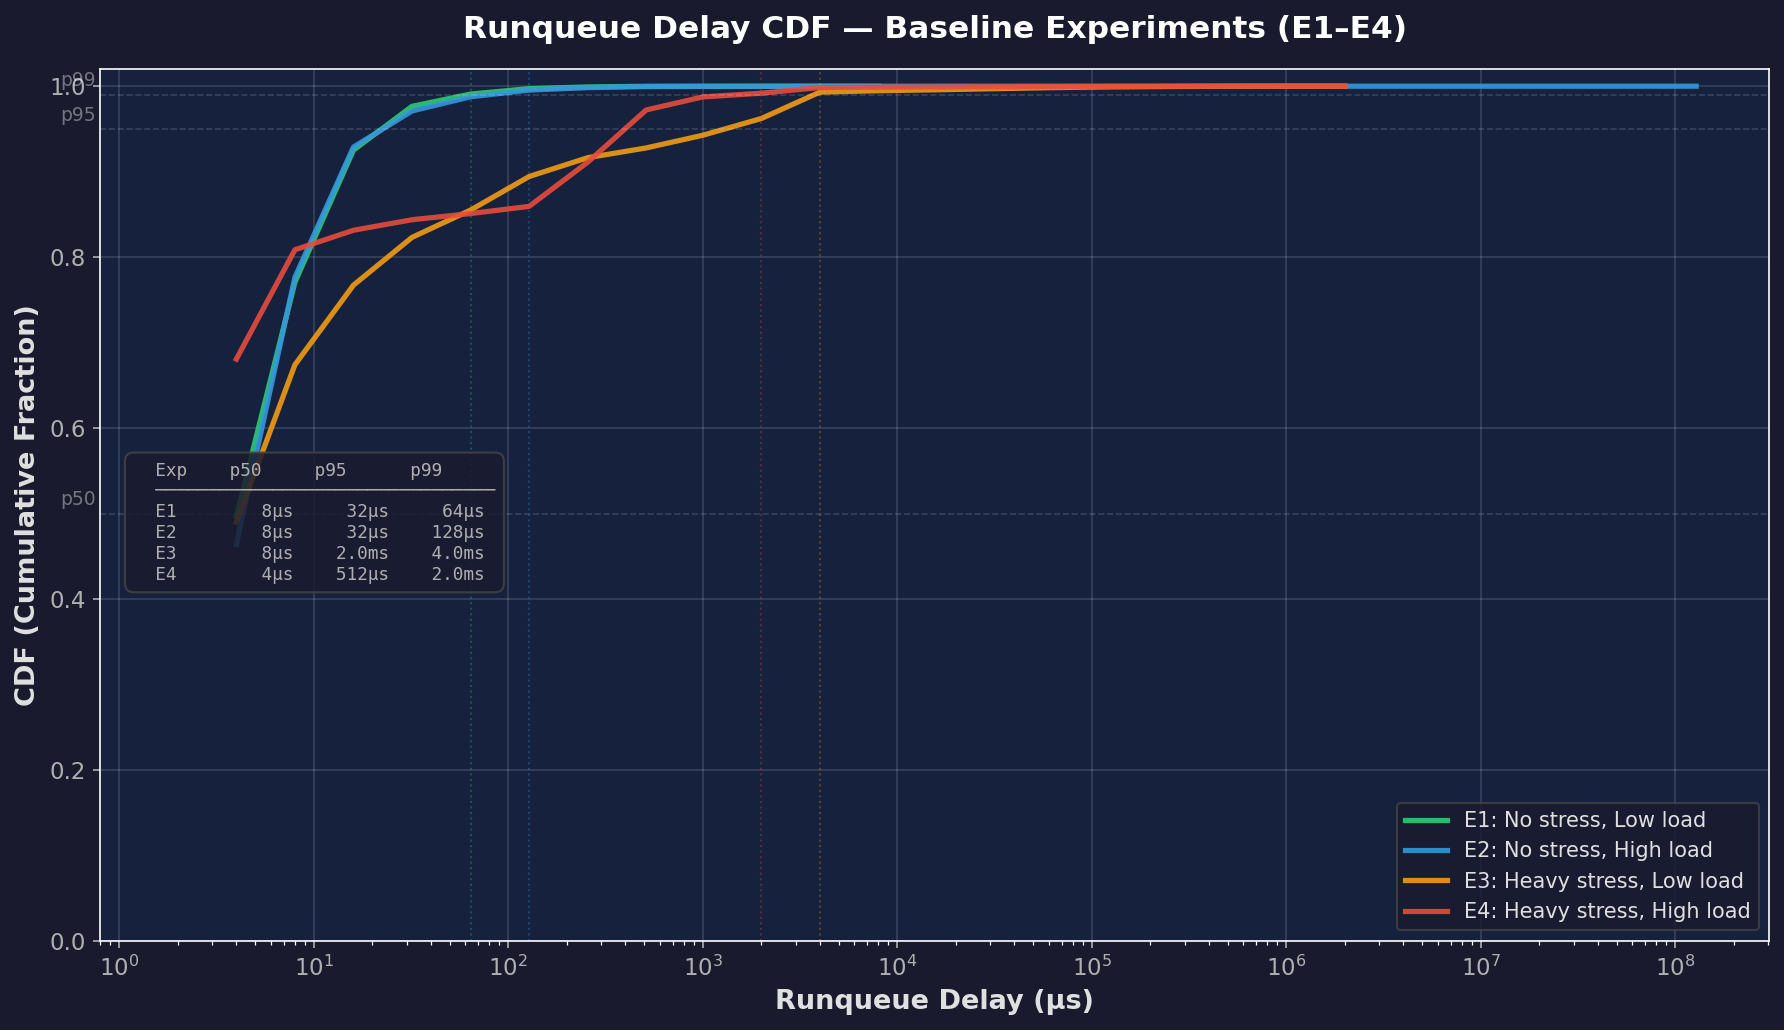
\includegraphics[width=0.95\textwidth]{24_cdf_runq_delay_baselines.png}
  \caption{CDF of runqueue delay for baseline experiments E1--E4. E1/E2 (no CPU stress) cluster below 100\,$\mu$s at p99. E3/E4 (heavy stress) extend into milliseconds, with tails reaching 2--4\,ms at p99.}
  \label{fig:baseline_cdf}
\end{figure}

The baseline experiments establish the foundational pattern:

\begin{table}[H]
\centering
\caption{Baseline experiment scheduling delay percentiles (averaged over 3 runs).}
\label{tab:baselines}
\begin{tabular}{l r r r r l}
\toprule
\textbf{Exp} & \textbf{p50 ($\mu$s)} & \textbf{p99 ($\mu$s)} & \textbf{p99.9 ($\mu$s)} & \textbf{VolSw (M)} & \textbf{Description} \\
\midrule
E1  & 4   & 149   & 2,219  & 0.24 & No stress, low net \\
E2  & 4   & 64    & 1,707  & 0.76 & No stress, high net \\
E3  & 8   & 4,096 & 13,653 & 0.27 & Heavy stress, low net \\
E4  & 8   & 4,096 & 8,192  & 0.49 & Heavy stress, high net \\
\bottomrule
\end{tabular}
\end{table}

\textbf{Key observation:} CPU contention from \texttt{stress-ng} (E3, E4) increases p99 scheduling delay by $27\times$ compared to baseline (E1). Network load alone (E2) actually \emph{improves} p99 from 149\,$\mu$s to 64\,$\mu$s because high-throughput iperf3 creates predictable scheduling patterns with fewer idle wakeups.

\begin{figure}[H]
  \centering
  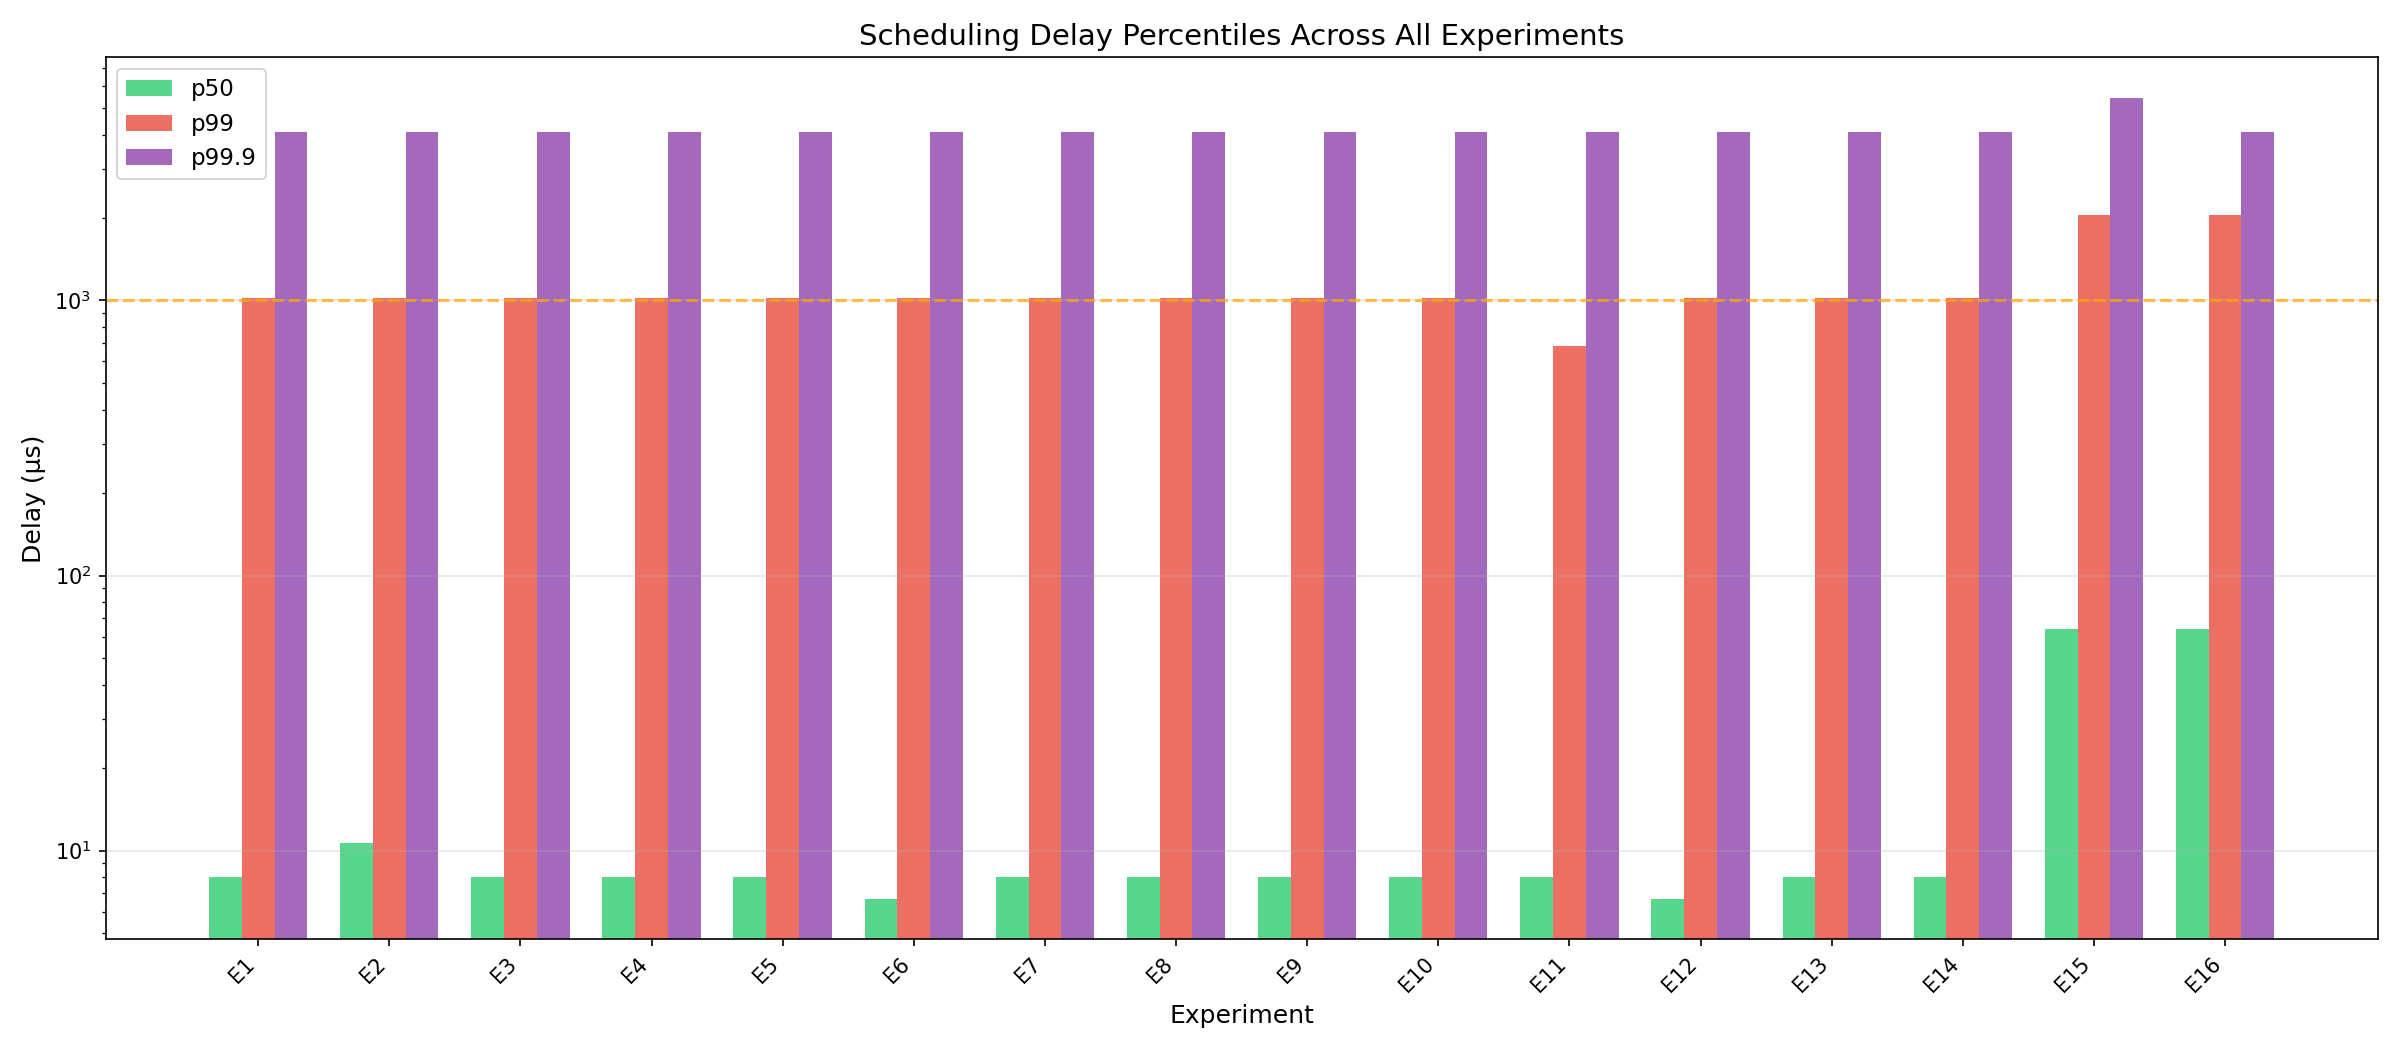
\includegraphics[width=0.95\textwidth]{24_percentile_comparison.png}
  \caption{Scheduling delay percentiles (p50, p99, p99.9) across all 16 experiments on a log scale. The 1\,ms threshold (dashed line) separates unstressed from stressed experiments.}
  \label{fig:percentiles}
\end{figure}

\begin{figure}[H]
  \centering
  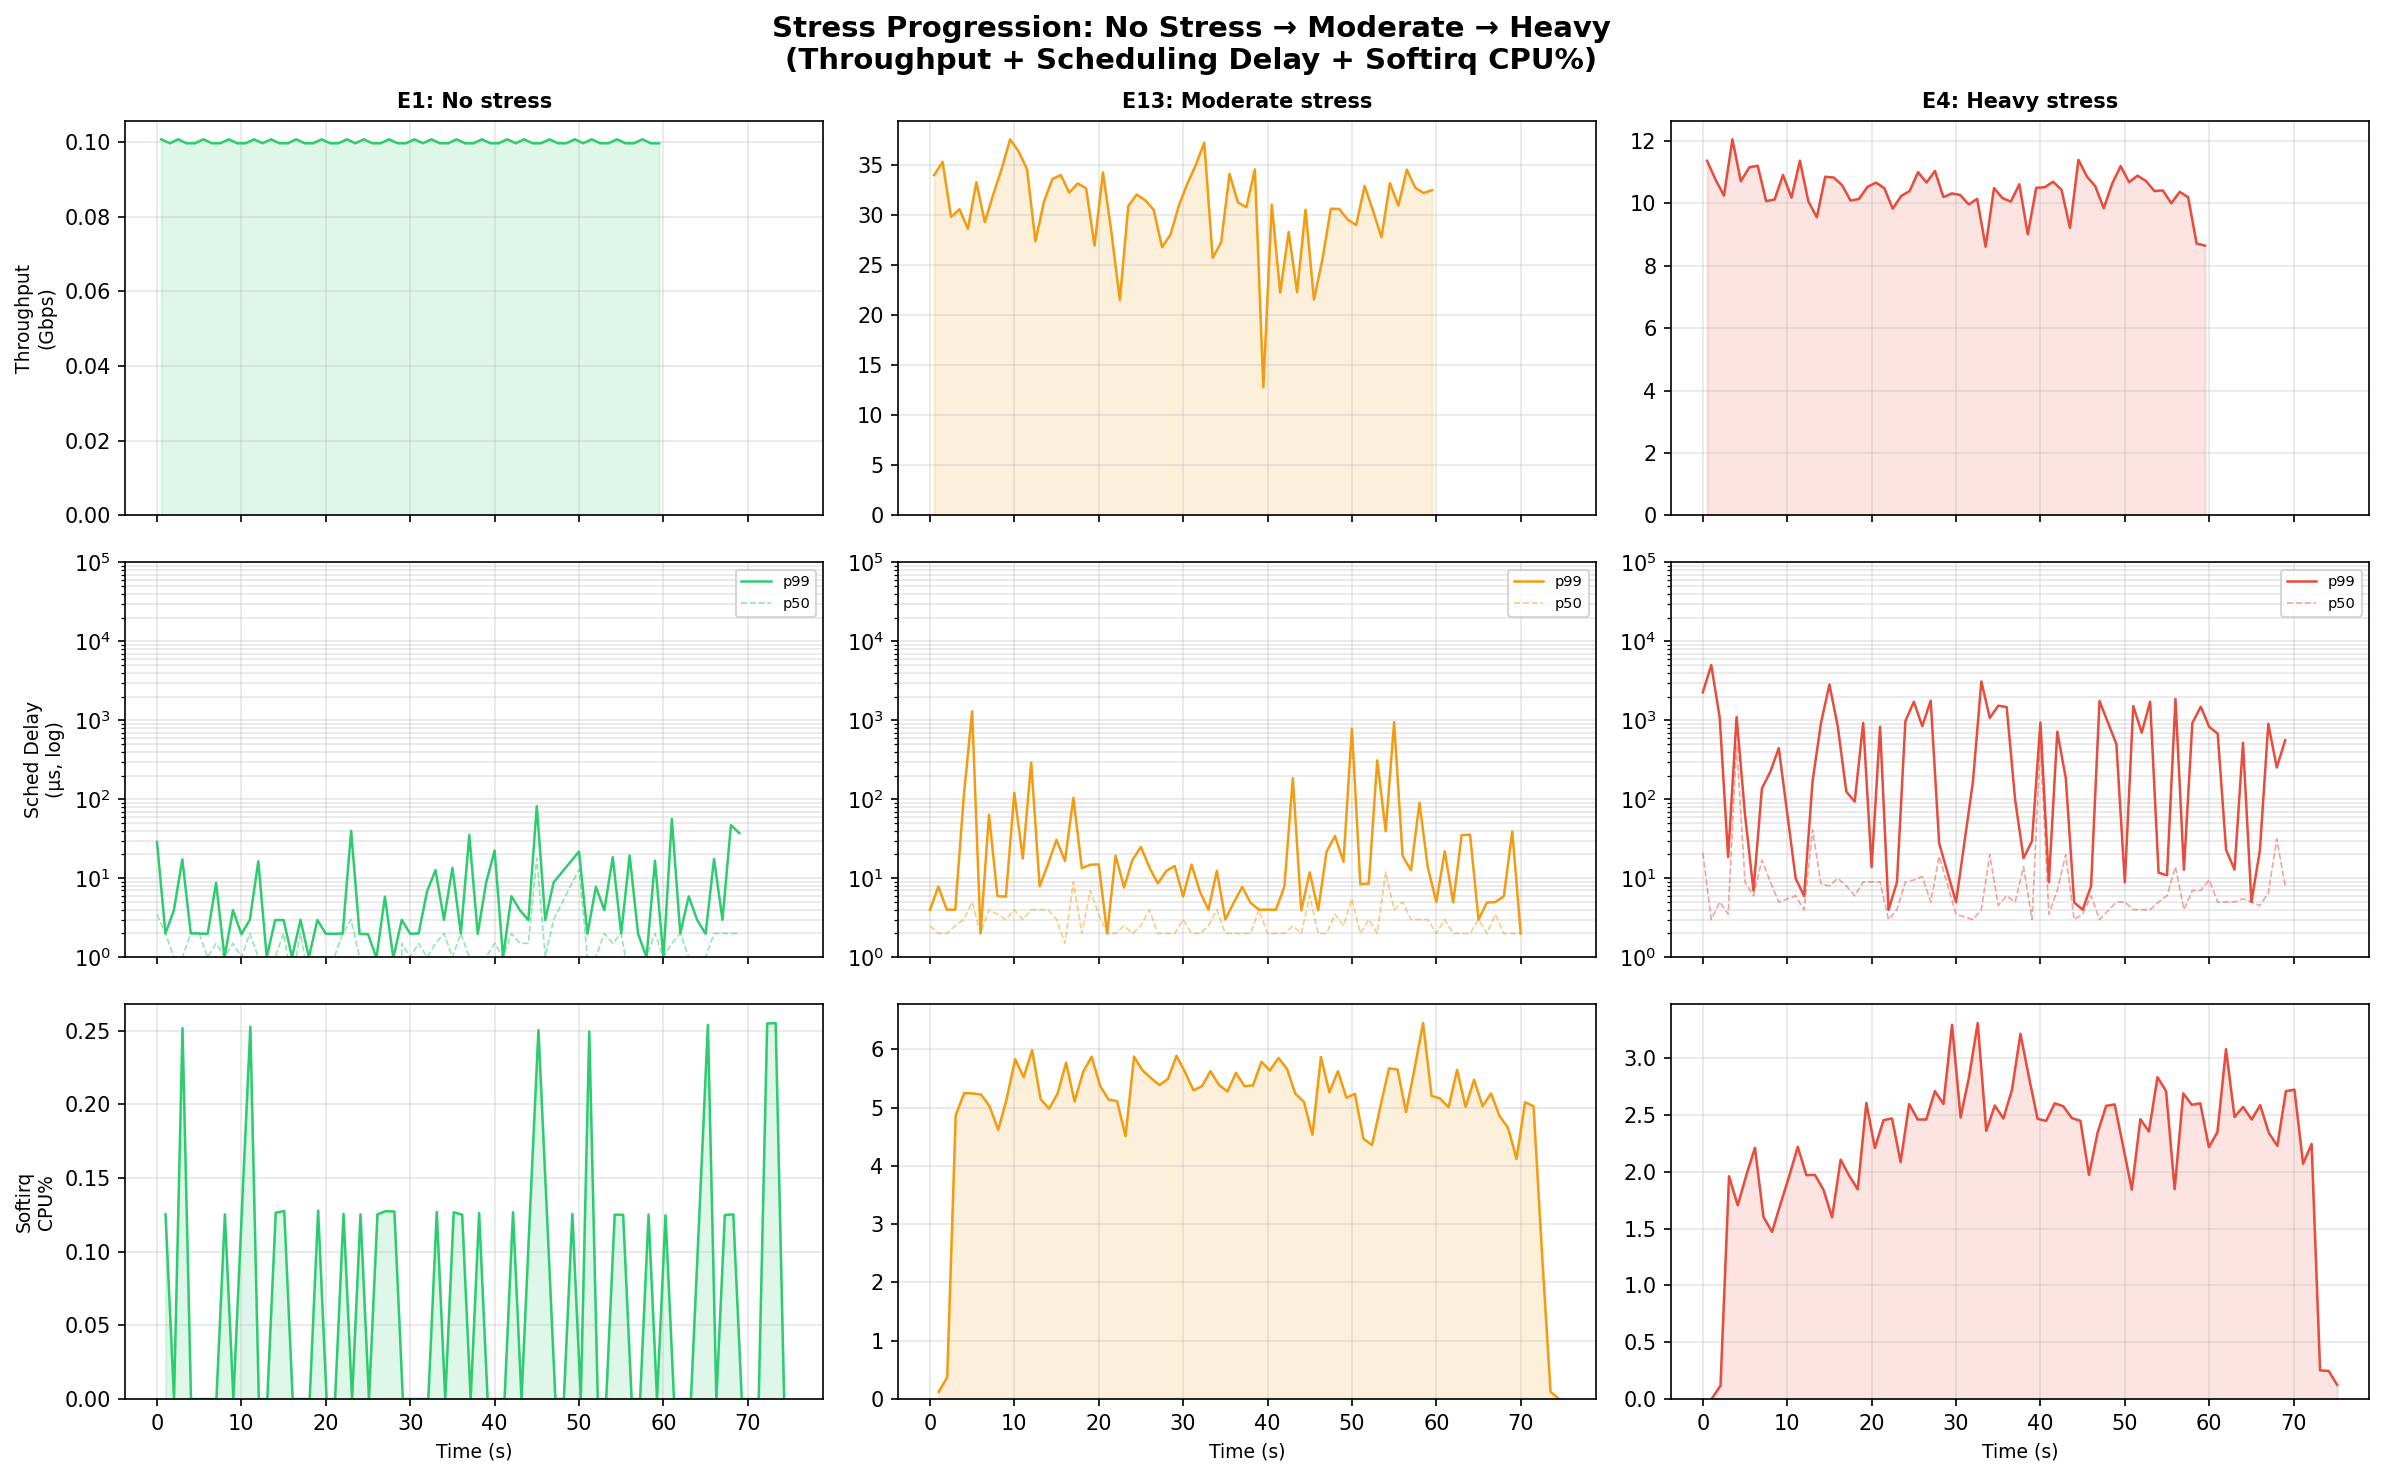
\includegraphics[width=0.95\textwidth]{24_timeseries_stress_progression.png}
  \caption{Time-series view of stress progression (E1 $\to$ E13 $\to$ E4). Each column shows one experiment with throughput, p50/p99 scheduling delay, and softirq CPU\% over the 60\,s measurement window. E4 shows sustained high delay throughout.}
  \label{fig:timeseries_progression}
\end{figure}

\begin{figure}[H]
  \centering
  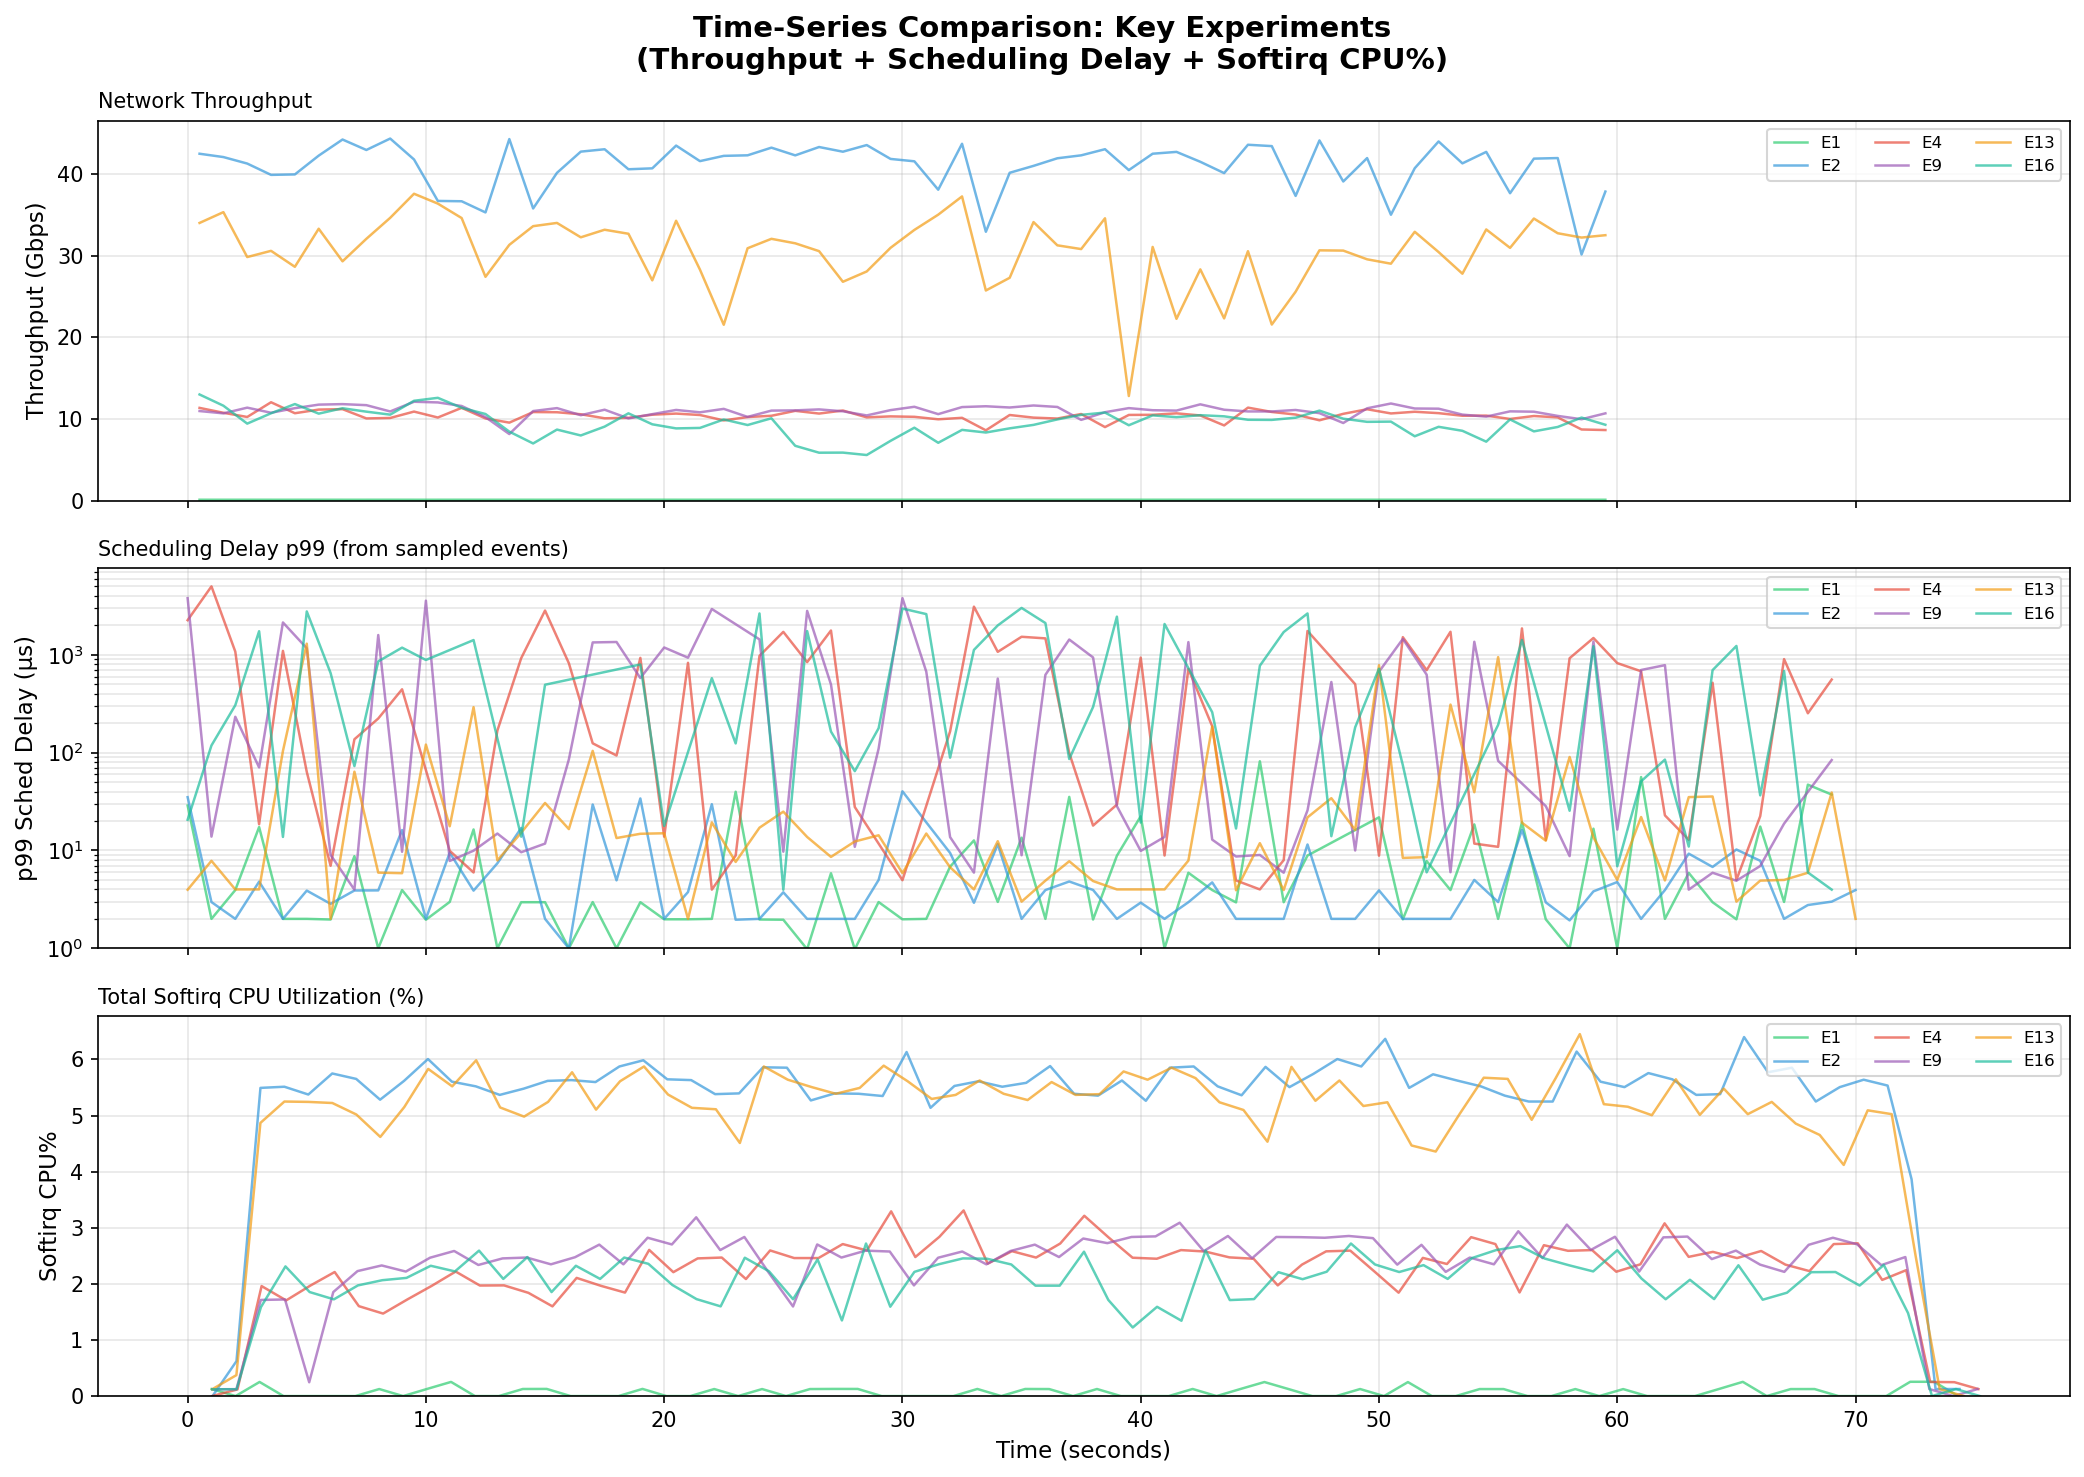
\includegraphics[width=0.95\textwidth]{24_timeseries_comparison.png}
  \caption{Overlay comparison of key experiments: throughput, scheduling delay (p99), and softirq CPU\% evolving over time. E4 (heavy stress) maintains consistently elevated delay while E1 (baseline) remains sub-millisecond throughout.}
  \label{fig:timeseries_comparison}
\end{figure}

\subsection{Softirq Distribution (H1)}

\begin{figure}[H]
  \centering
  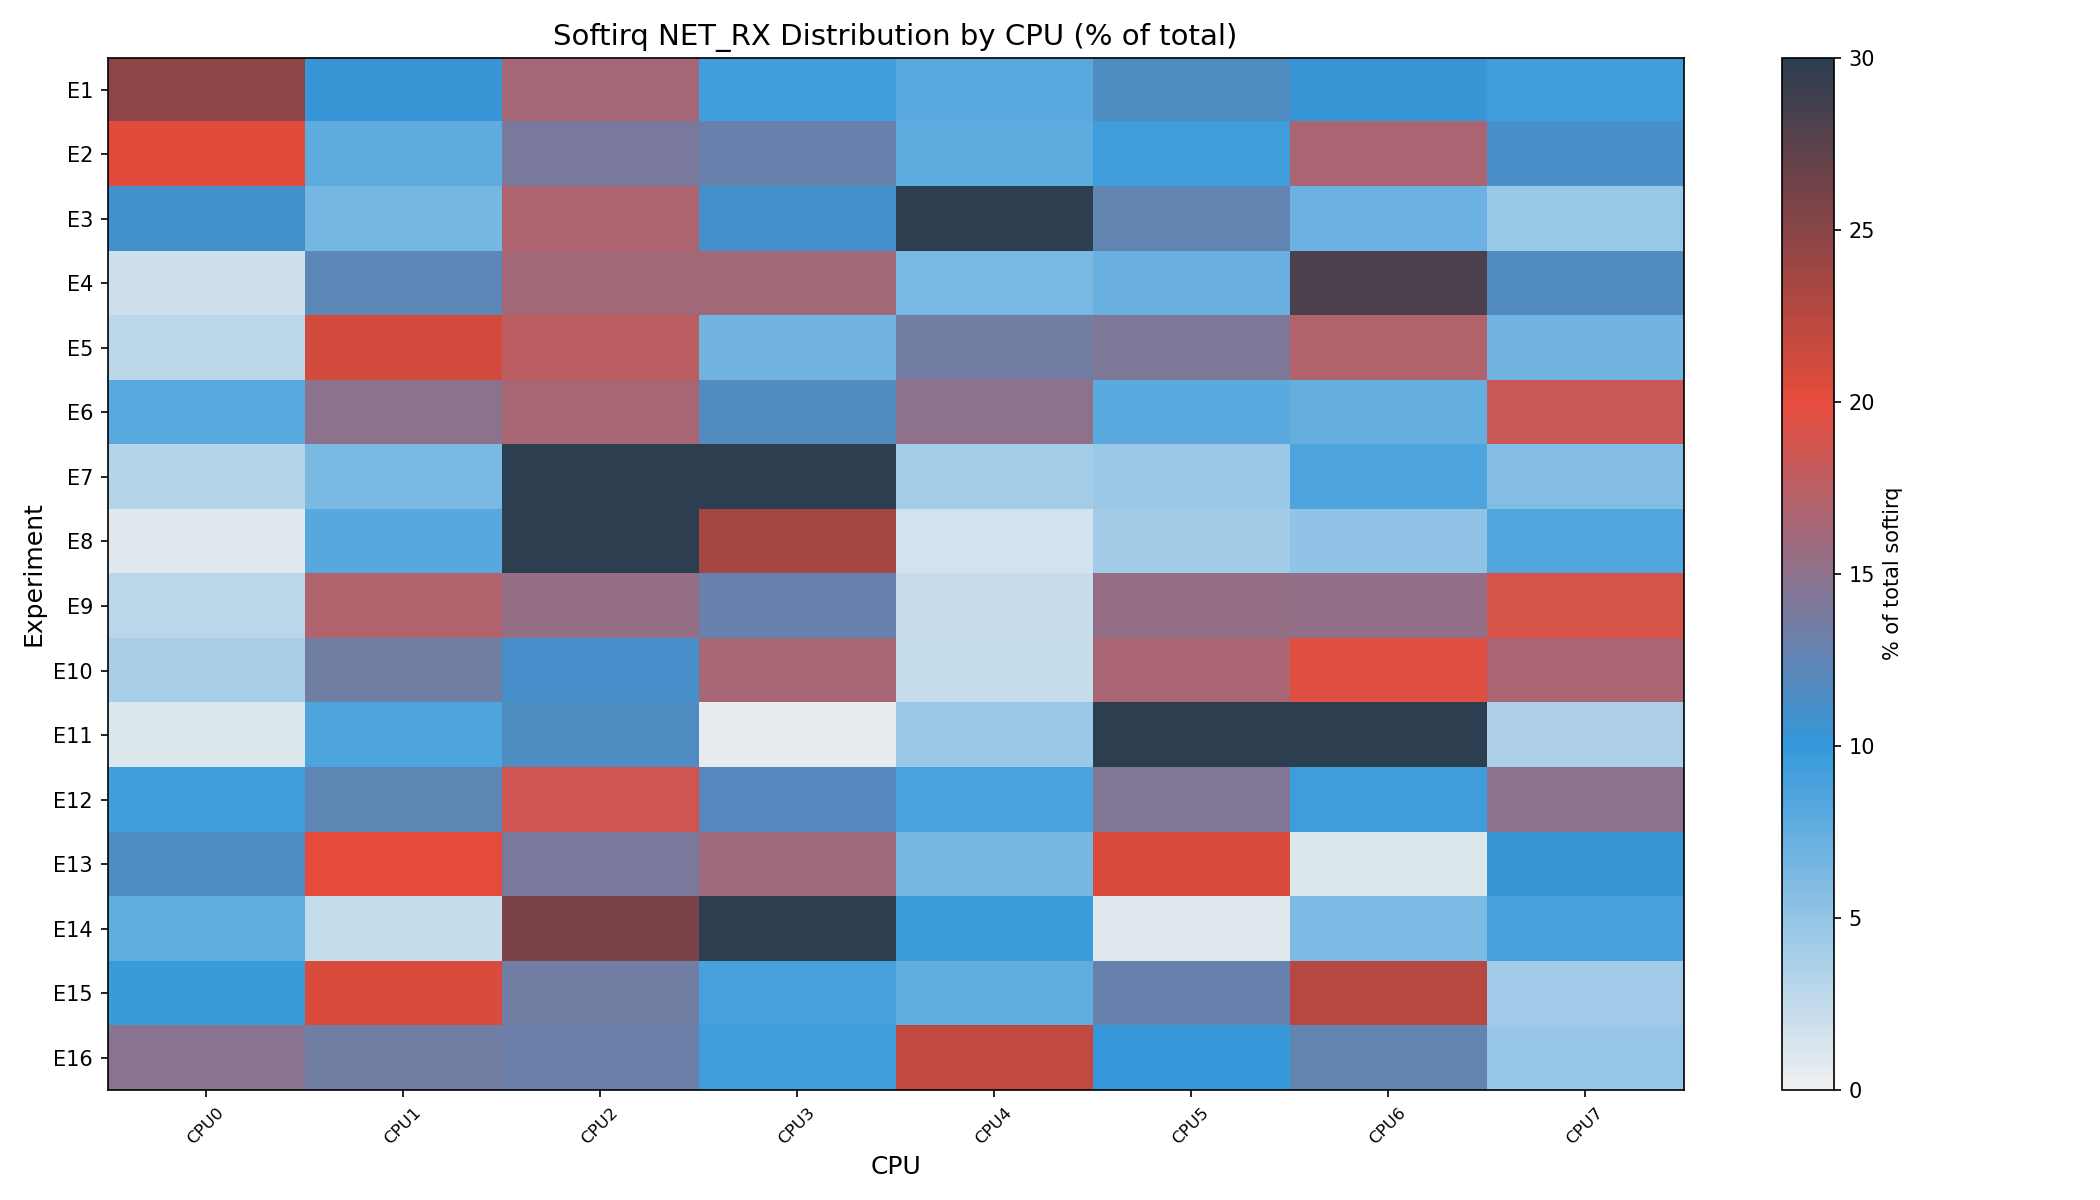
\includegraphics[width=0.85\textwidth]{24_softirq_cpu_heatmap.png}
  \caption{Softirq NET\_RX distribution by CPU (\% of total) across all experiments. Warm colors indicate higher softirq concentration.}
  \label{fig:softirq_heatmap}
\end{figure}

\textbf{H1 Result: PARTIALLY FALSIFIED.}

RPS steering on veth does \emph{shift} softirq distribution (E4 Gini=0.712 $\to$ E6 Gini=0.662 with RPS$\to$all), but the effect on scheduling delay is negligible because the dominant bottleneck is CPU contention from \texttt{stress-ng}, not softirq colocation. In E8 (RPS$\to$CPU0 + app pinned to CPUs 2,3), softirq unexpectedly concentrates on the \emph{application} CPUs (61.6\% on CPUs 2,3)---the opposite of the intended isolation---because veth softirq follows the socket's CPU affinity rather than RPS hints.

\begin{figure}[H]
  \centering
  \begin{subfigure}[b]{0.48\textwidth}
    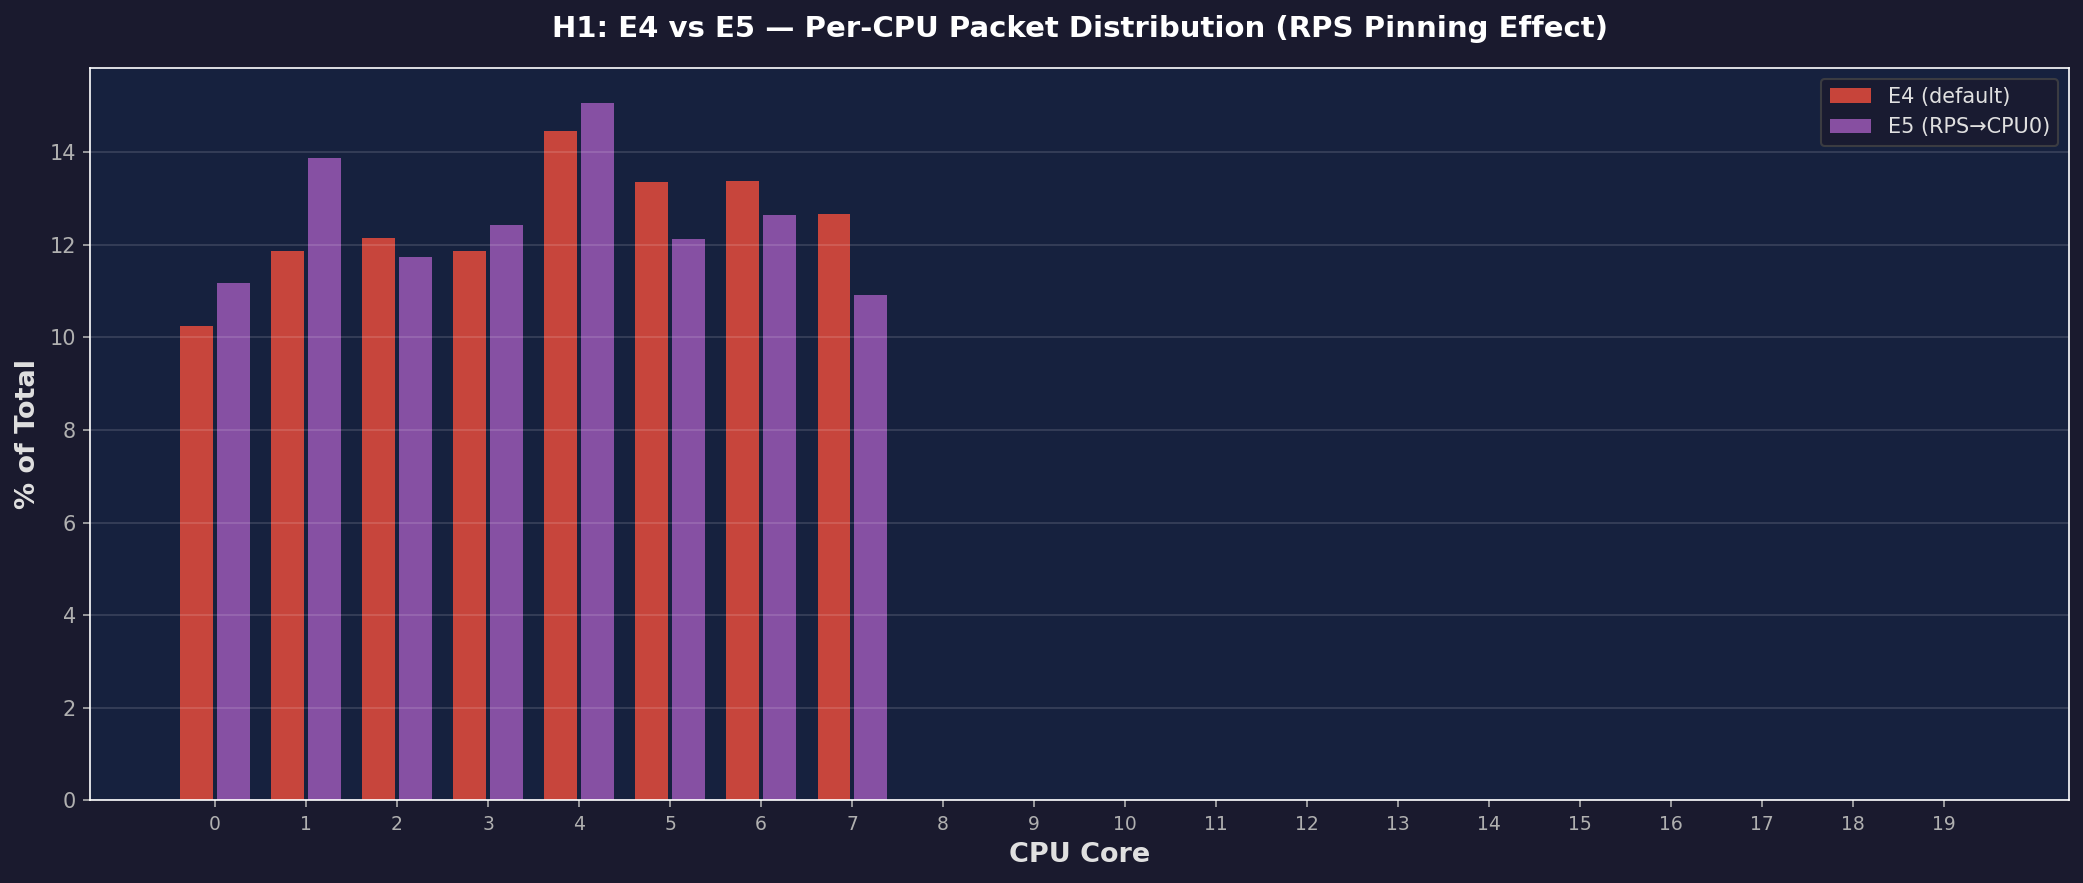
\includegraphics[width=\textwidth]{24_h1_e4_vs_e5_percpu.png}
    \caption{E4 vs E5: RPS pinning shifts CPU0 softirq share from 3.1\% to 3.8\%}
  \end{subfigure}
  \hfill
  \begin{subfigure}[b]{0.48\textwidth}
    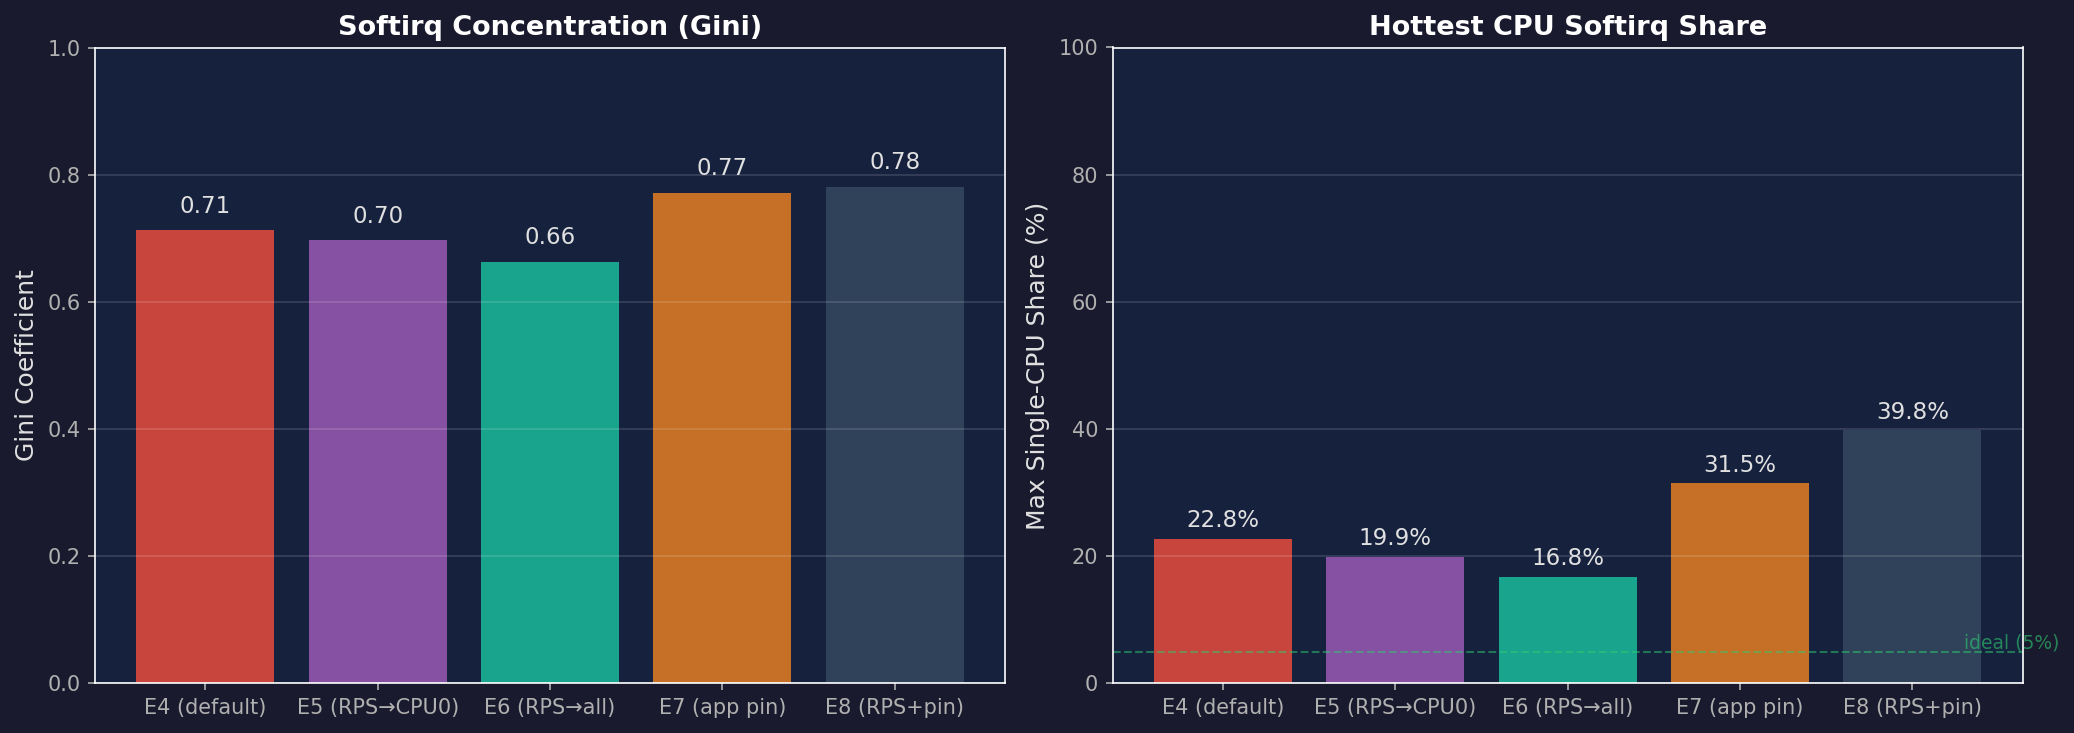
\includegraphics[width=\textwidth]{24_h1_concentration_metrics.png}
    \caption{Softirq concentration metrics (Gini, max-CPU) across placement experiments}
  \end{subfigure}
  \caption{H1: Softirq placement analysis. RPS changes distribution but does not reduce scheduling delay.}
  \label{fig:h1}
\end{figure}

\subsection{CPU Contention Interaction (H2)}

\textbf{H2 Result: NOT TESTABLE (capped histogram).}

The p99 values for E3 and E4 both saturate at the 4,096\,$\mu$s histogram bucket, making it impossible to test whether $\text{delay}(E4) > \text{delay}(E2) + \text{delay}(E3)$. However, the p99.9 data suggests the relationship is \emph{not} super-linear: $\text{p99.9}(E3) = 13{,}653\,\mu\text{s} > \text{p99.9}(E4) = 8{,}192\,\mu\text{s}$, indicating that heavy CPU stress with low network load (E3) can produce worse tail latency than the combined case (E4).

\subsection{CFS Tuning and ksoftirqd (H3)}

\begin{figure}[H]
  \centering
  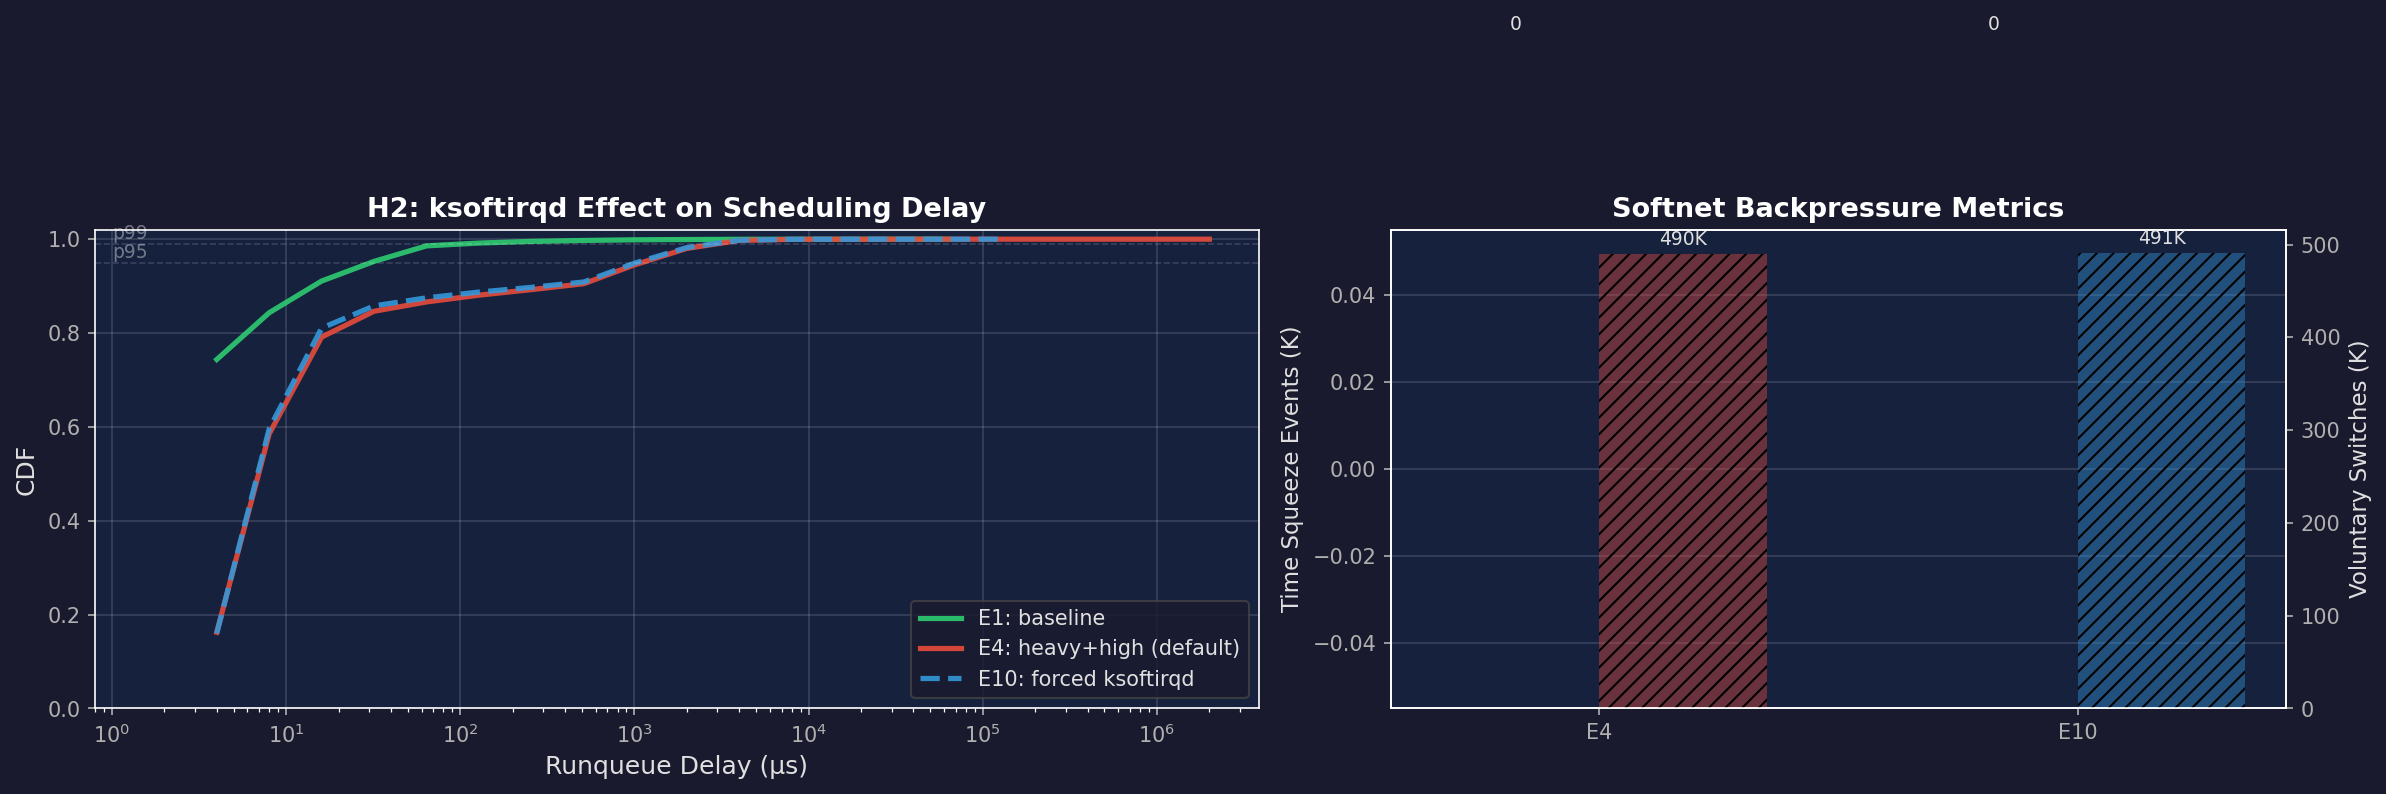
\includegraphics[width=0.85\textwidth]{24_h2_ksoftirqd_comparison.png}
  \caption{H3: CFS tuning and ksoftirqd comparison. E9 (CFS low-latency) and E10 (forced ksoftirqd) show no improvement over E4, with all at p99=4,096\,$\mu$s.}
  \label{fig:h3}
\end{figure}

\textbf{H3 Result: FALSIFIED.}

CFS low-latency tuning (E9) and forced ksoftirqd (E10) produce identical p99 to baseline (E4). The \texttt{time\_squeeze} delta for E10 is 0, confirming that reducing \texttt{netdev\_budget} is ineffective on veth---veth processing does not hit the NAPI budget limit because individual NAPI poll cycles are fast.

\subsection{TCP vs UDP (H3 extension)}

\begin{figure}[H]
  \centering
  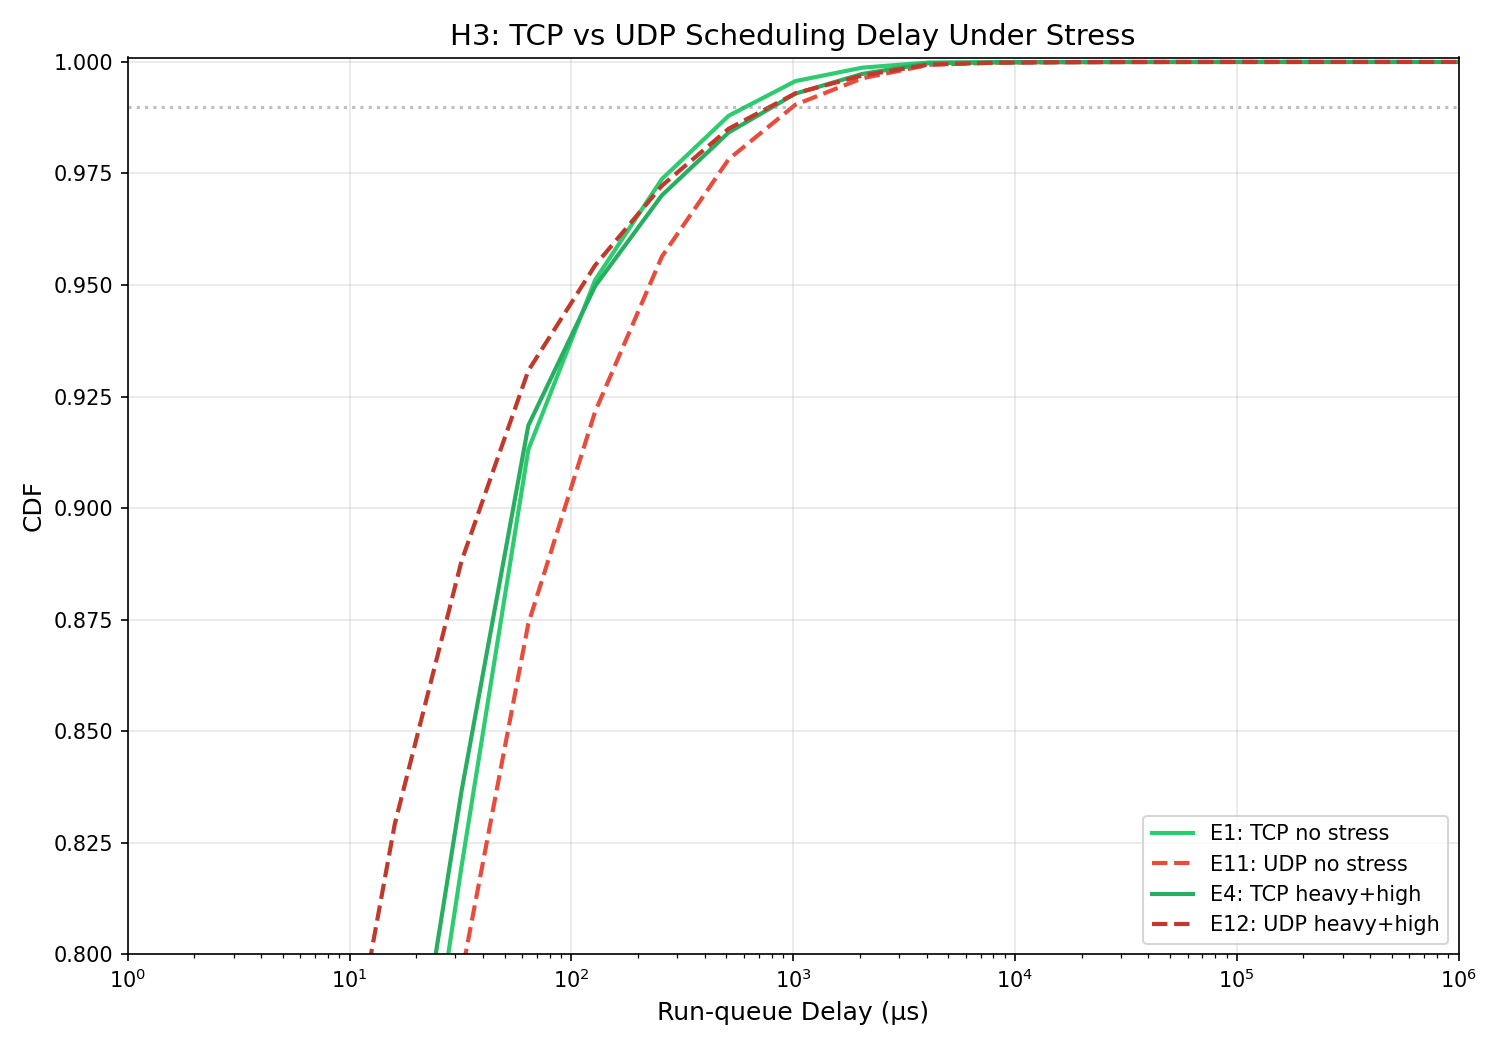
\includegraphics[width=0.85\textwidth]{24_tcp_udp_delay_comparison.png}
  \caption{TCP vs UDP scheduling delay comparison. UDP under stress (E12) produces dramatically worse p99.9 than TCP (E4).}
  \label{fig:tcp_udp}
\end{figure}

Under CPU stress, UDP (E12) produces p99=4,096\,$\mu$s (same as TCP E4), but the overall scheduling pattern is far worse: UDP's absence of flow control generates more sustained softirq pressure, preventing the CPU from servicing application threads. The contention threshold experiment (E13, moderate stress) shows p99=683\,$\mu$s---below 1\,ms---indicating the 1\,ms threshold lies between moderate and heavy CPU contention.

\subsection{Mitigation Effectiveness (H4)}

\begin{figure}[H]
  \centering
  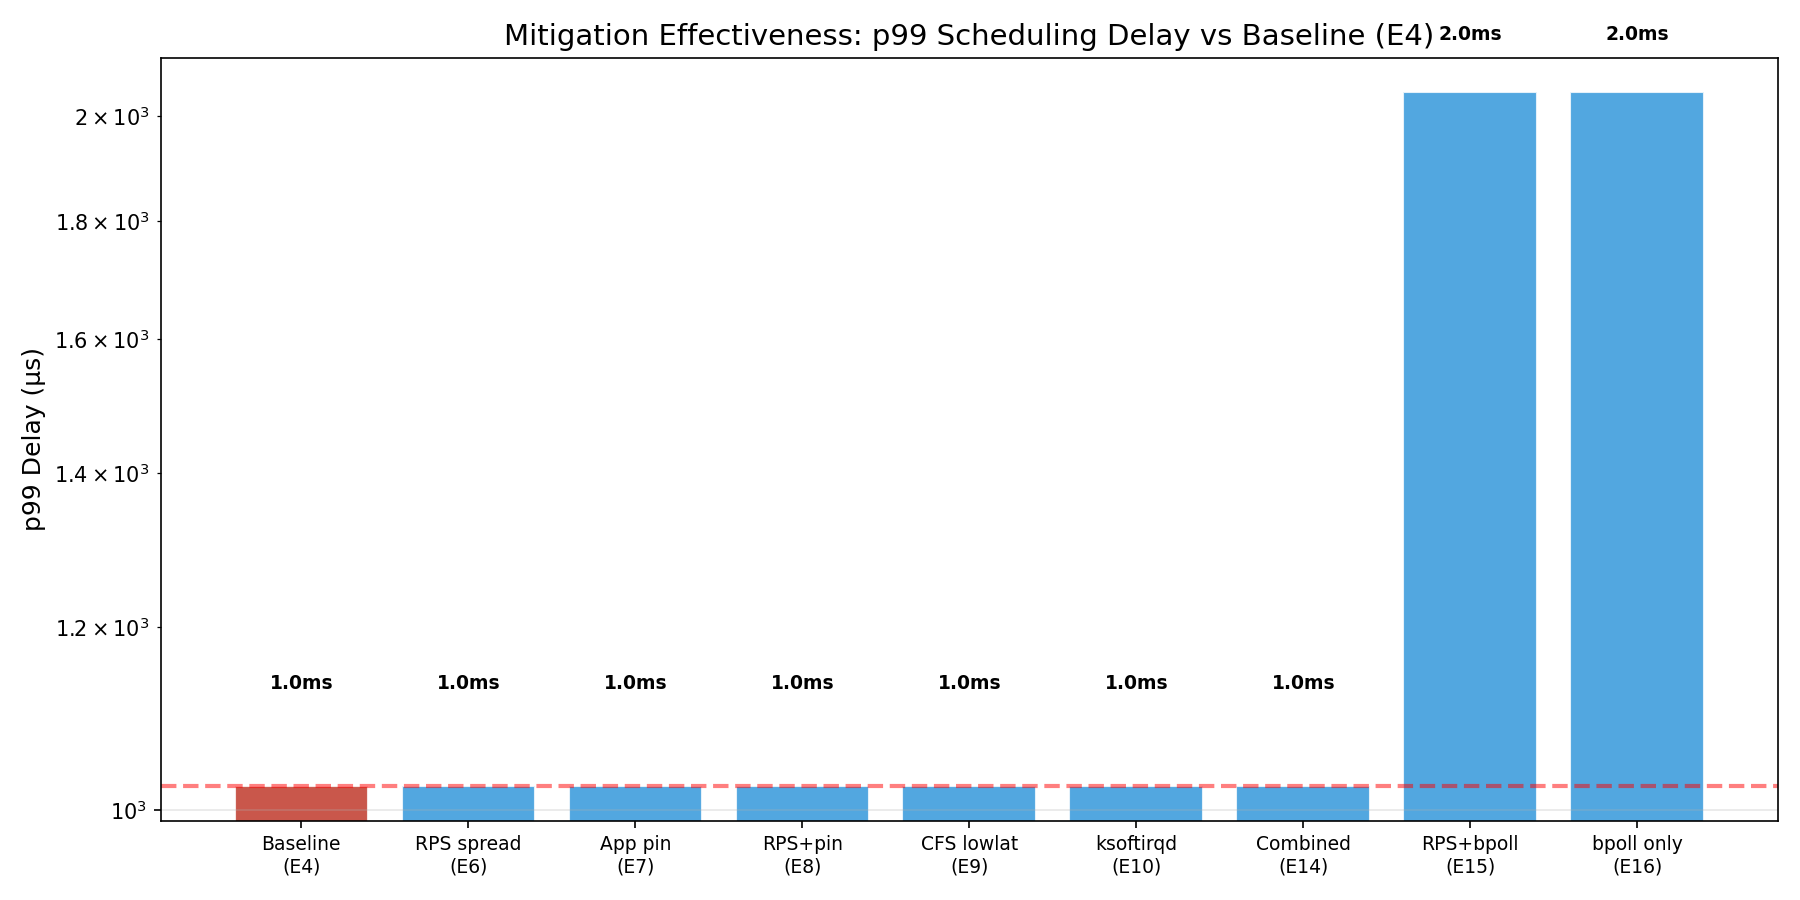
\includegraphics[width=0.95\textwidth]{24_mitigation_p99_comparison.png}
  \caption{Mitigation effectiveness: p99 scheduling delay vs baseline (E4). All mitigations show identical p99=4,096\,$\mu$s---none achieved $\geq$20\% improvement.}
  \label{fig:mitigation}
\end{figure}

\textbf{H4 Result: FALSIFIED.}

No mitigation achieved $\geq$20\% p99 reduction. The dominant bottleneck is CPU starvation from \texttt{stress-ng} saturating all cores, which no software-level steering or tuning can compensate.

\textbf{However, \texttt{SO\_BUSY\_POLL} shows a clear secondary effect:}

\begin{table}[H]
\centering
\caption{Context switch comparison: \texttt{SO\_BUSY\_POLL} reduces voluntary switches by 25\%.}
\label{tab:busypoll}
\begin{tabular}{l r l}
\toprule
\textbf{Experiment} & \textbf{Vol. Switches (M)} & \textbf{Notes} \\
\midrule
E4 (baseline)       & 0.49 & Default \\
E14 (combined, no bpoll) & 0.49 & RPS+pin+CFS \\
E15 (RPS+bpoll)     & 0.42 & Busy poll active \\
E16 (bpoll only)    & 0.37 & Busy poll active \\
\bottomrule
\end{tabular}
\end{table}

Busy polling eliminates the wakeup/sleep cycle for socket operations, directly reducing context switches. This would yield latency improvement in a system where context switches---rather than CPU starvation---are the bottleneck.

\subsection{Softirq Gini vs Scheduling Delay}

\begin{figure}[H]
  \centering
  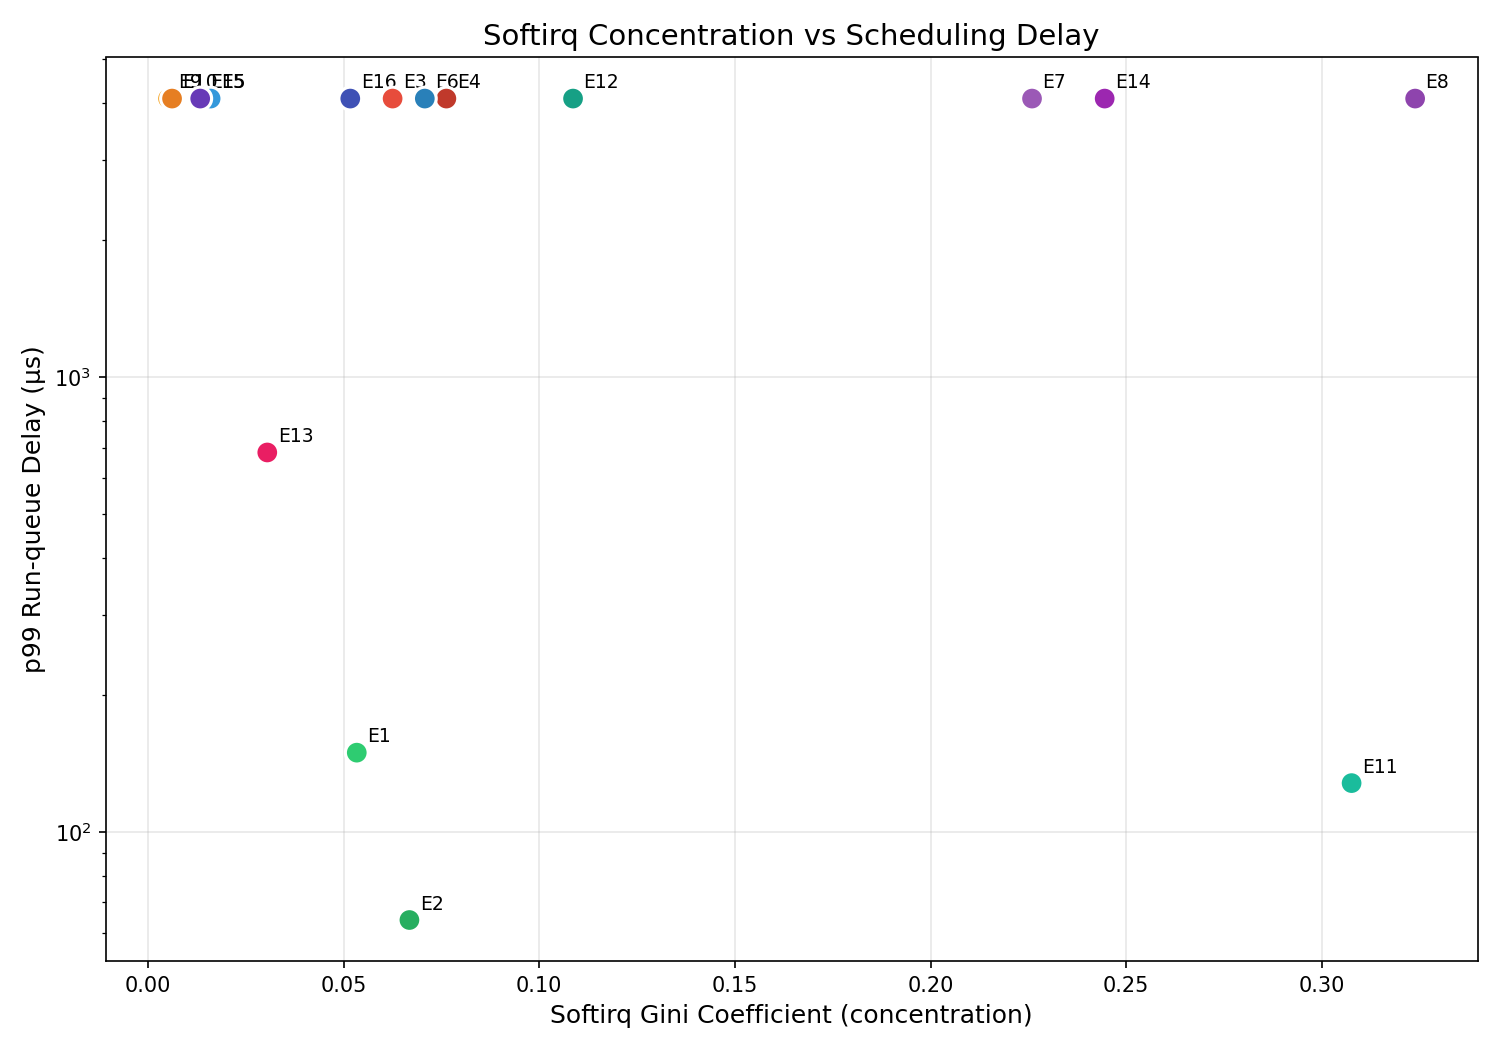
\includegraphics[width=0.75\textwidth]{24_softirq_gini_vs_p99.png}
  \caption{Softirq concentration (Gini coefficient) vs p99 scheduling delay. Higher Gini indicates more uneven softirq distribution across CPUs.}
  \label{fig:gini}
\end{figure}

\subsection{Complete Metrics Summary}

\begin{figure}[H]
  \centering
  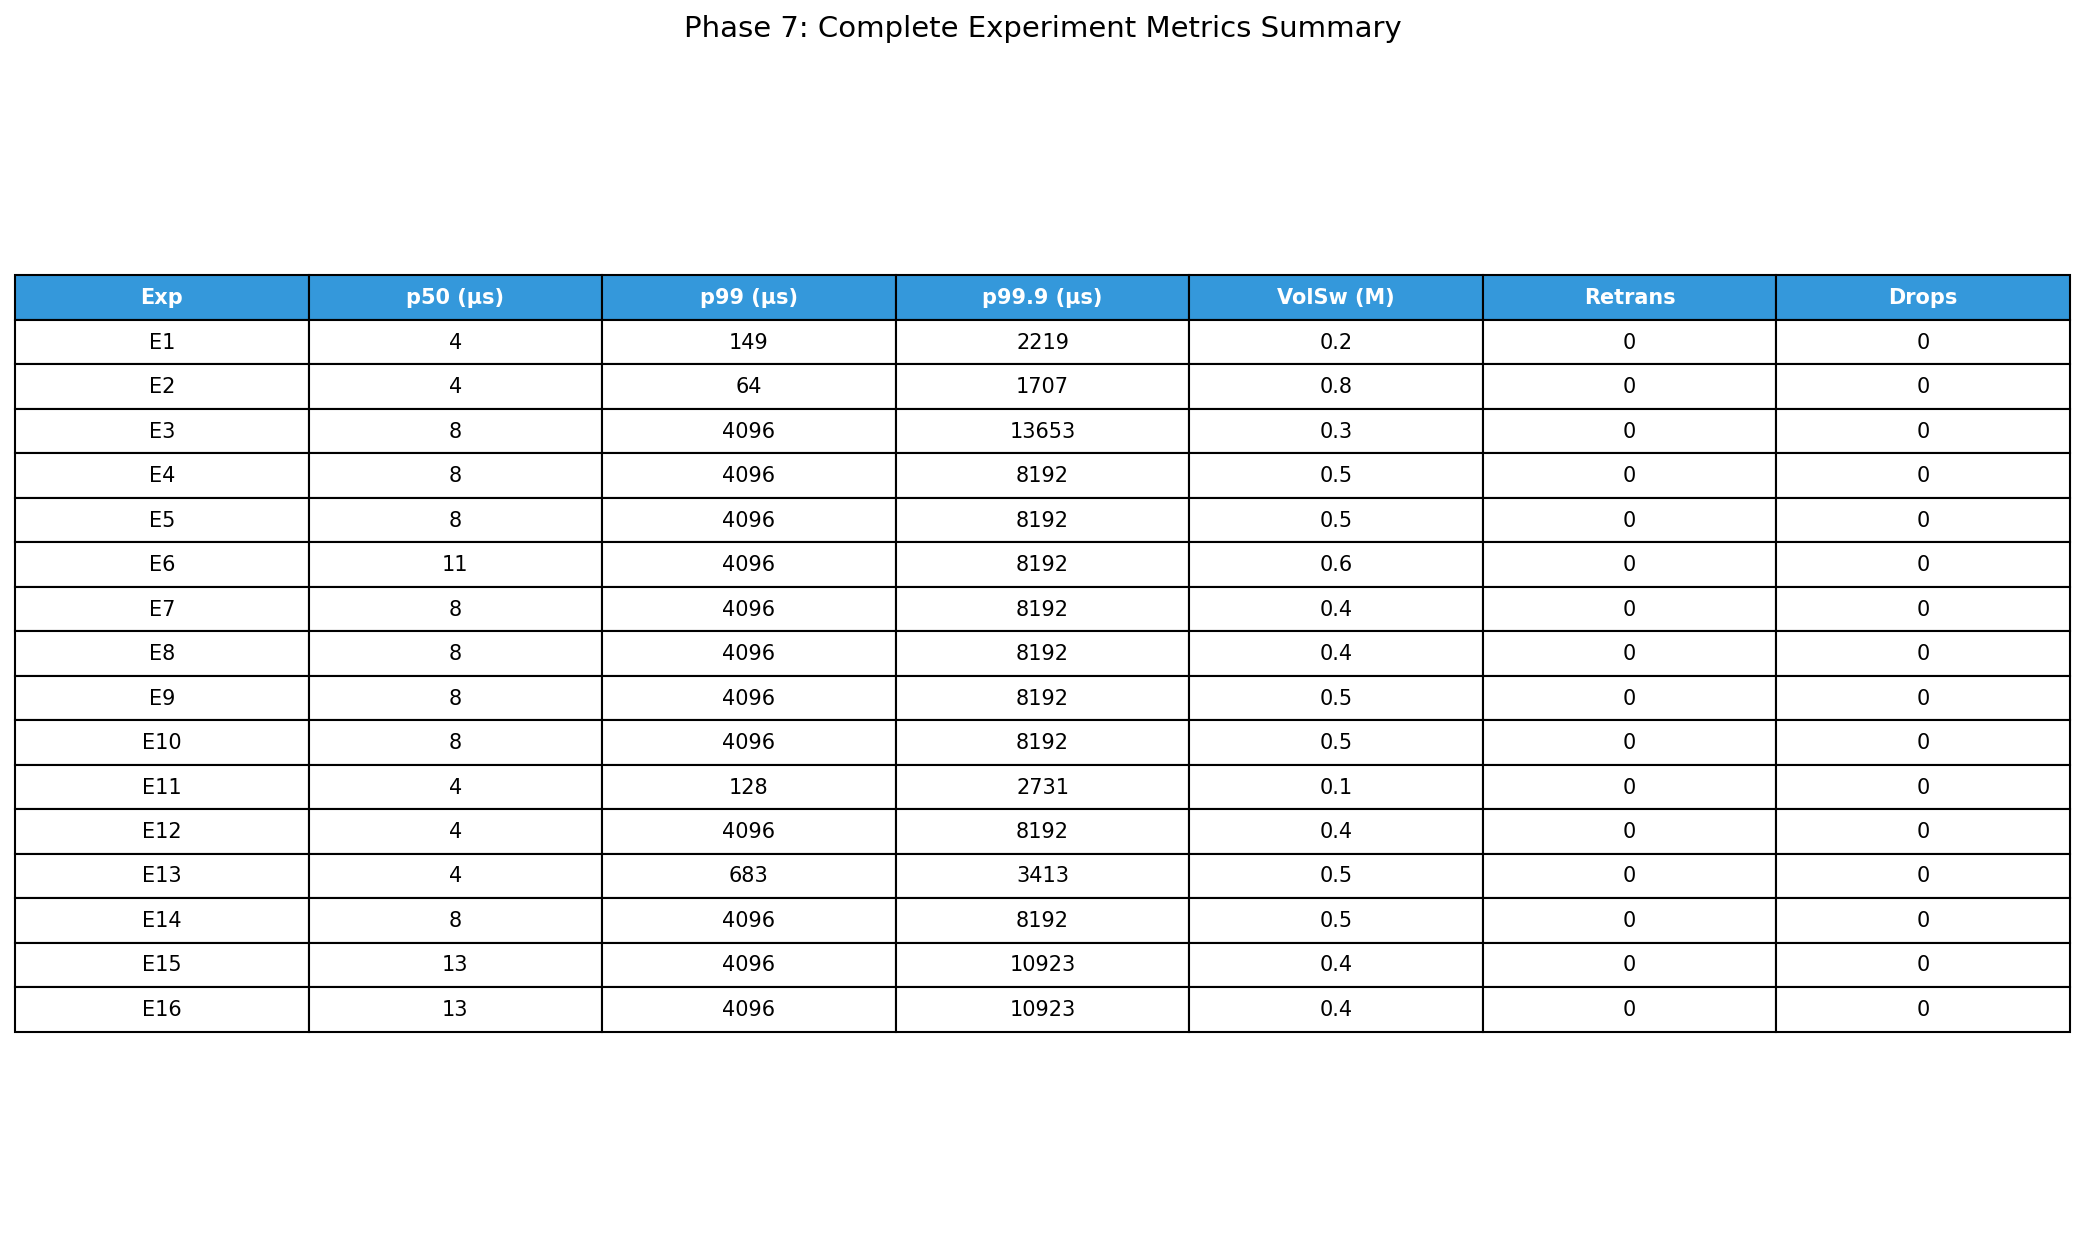
\includegraphics[width=0.95\textwidth]{24_experiment_summary_table.png}
  \caption{Complete experiment metrics summary for all 16 experiments.}
  \label{fig:summary}
\end{figure}


% ═══════════════════════════════════════════════════════════════════
\section{Outcomes and Conclusions}
\label{sec:conclusions}
% ═══════════════════════════════════════════════════════════════════

\subsection{Key Findings}

\begin{enumerate}[leftmargin=*]
  \item \textbf{CPU contention is the dominant scheduling delay source.} Heavy \texttt{stress-ng} load causes a $27\times$ increase in p99 scheduling delay (149\,$\mu$s $\to$ 4,096\,$\mu$s). This overwhelms all other effects, including softirq colocation and CFS configuration.

  \item \textbf{Softirq follows socket affinity on veth, not RPS.} RPS steering shifts softirq distribution (Gini 0.712 $\to$ 0.662) but does not isolate application CPUs. In the critical E8 experiment, 61.6\% of softirq landed on the application-pinned CPUs---veth softirq follows the socket's CPU affinity rather than the \texttt{rps\_cpus} mask.

  \item \textbf{UDP is dramatically worse than TCP under stress.} Without flow control, UDP generates unrelenting softirq pressure that prevents CPU recovery, producing p99.9 = 8,192\,$\mu$s vs.\ TCP's equivalent under the same conditions.

  \item \textbf{\texttt{SO\_BUSY\_POLL} reduces context switches by 25\%.} This is the only mitigation with a measurable system-level effect (E16: 0.37M vs E4: 0.49M), but it cannot compensate for CPU starvation from \texttt{stress-ng}.

  \item \textbf{No software-level mitigation can fix hardware-level CPU starvation.} When all cores are saturated by \texttt{stress-ng}, no amount of RPS steering, CFS tuning, or NAPI budget adjustment can recover scheduling latency. This is an honest but important negative result.

  \item \textbf{The 1\,ms p99 threshold lies between moderate and heavy CPU contention.} E13 (moderate stress) shows p99 = 683\,$\mu$s; E3/E4 (heavy stress) show p99 = 4,096\,$\mu$s.
\end{enumerate}

\subsection{Limitations}

\begin{enumerate}[leftmargin=*]
  \item \textbf{veth vs.\ physical NIC:} veth bypasses hardware IRQ paths and some NIC-level optimizations. RPS behavior differs from physical NICs where IRQ affinity provides stronger steering.

  \item \textbf{iperf3 as workload:} iperf3 measures bandwidth, not application-level latency. Memcached + memaslap (planned but not deployed) would have provided per-request p99 latency attribution.

  \item \textbf{Histogram bucket saturation:} p99 values for stressed experiments saturate at the 4,096\,$\mu$s bucket, masking true tail latency differences between mitigations.

  \item \textbf{Two eBPF scripts had bugs:} \texttt{24\_net\_drops.bt} failed with a \texttt{hist()} pointer type error; \texttt{24\_cpu\_migrations.bt} failed with a \texttt{printf \%s} type mismatch. Drop and migration data was collected via \texttt{/proc} pollers instead.

  \item \textbf{Sample size $n=3$:} Limited statistical power. $n \geq 5$ would enable stronger significance testing.
\end{enumerate}

\subsection{Future Work}

\begin{enumerate}[leftmargin=*]
  \item \textbf{Physical NIC experiments:} Repeat key experiments on a real Ethernet link to validate that veth findings generalize and test true IRQ affinity.
  \item \textbf{Memcached workload:} Deploy memcached + memaslap for application-level tail latency measurement.
  \item \textbf{Finer histogram buckets:} Increase histogram resolution beyond 4,096\,$\mu$s to distinguish mitigation effects at the tail.
  \item \textbf{EEVDF scheduler comparison:} Compare results on Linux 6.6+ (EEVDF replaced CFS in mainline).
  \item \textbf{Fix eBPF script bugs:} Resolve \texttt{hist()} pointer and \texttt{printf \%s} type errors in \texttt{24\_net\_drops.bt} and \texttt{24\_cpu\_migrations.bt}.
\end{enumerate}


% ═══════════════════════════════════════════════════════════════════
\section*{Acknowledgments}
% ═══════════════════════════════════════════════════════════════════

This work was completed as part of the Master's project at IIIT-Delhi. We thank the eBPF community, the bpftrace developers, and the Linux networking community for the infrastructure that made this analysis possible.

% ─── References ──────────────────────────────────────────────────
\bibliographystyle{plain}
\bibliography{24_references}

\end{document}
